\documentclass[twoside]{book}

% Packages required by doxygen
\usepackage{fixltx2e}
\usepackage{calc}
\usepackage{doxygen}
\usepackage{graphicx}
\usepackage[utf8]{inputenc}
\usepackage{makeidx}
\usepackage{multicol}
\usepackage{multirow}
\PassOptionsToPackage{warn}{textcomp}
\usepackage{textcomp}
\usepackage[nointegrals]{wasysym}
\usepackage[table]{xcolor}

% Font selection
\usepackage[T1]{fontenc}
\usepackage[scaled=.90]{helvet}
\usepackage{courier}
\usepackage{amssymb}
\usepackage{sectsty}
\renewcommand{\familydefault}{\sfdefault}
\allsectionsfont{%
  \fontseries{bc}\selectfont%
  \color{darkgray}%
}
\renewcommand{\DoxyLabelFont}{%
  \fontseries{bc}\selectfont%
  \color{darkgray}%
}
\newcommand{\+}{\discretionary{\mbox{\scriptsize$\hookleftarrow$}}{}{}}

% Page & text layout
\usepackage{geometry}
\geometry{%
  a4paper,%
  top=2.5cm,%
  bottom=2.5cm,%
  left=2.5cm,%
  right=2.5cm%
}
\tolerance=750
\hfuzz=15pt
\hbadness=750
\setlength{\emergencystretch}{15pt}
\setlength{\parindent}{0cm}
\setlength{\parskip}{0.2cm}
\makeatletter
\renewcommand{\paragraph}{%
  \@startsection{paragraph}{4}{0ex}{-1.0ex}{1.0ex}{%
    \normalfont\normalsize\bfseries\SS@parafont%
  }%
}
\renewcommand{\subparagraph}{%
  \@startsection{subparagraph}{5}{0ex}{-1.0ex}{1.0ex}{%
    \normalfont\normalsize\bfseries\SS@subparafont%
  }%
}
\makeatother

% Headers & footers
\usepackage{fancyhdr}
\pagestyle{fancyplain}
\fancyhead[LE]{\fancyplain{}{\bfseries\thepage}}
\fancyhead[CE]{\fancyplain{}{}}
\fancyhead[RE]{\fancyplain{}{\bfseries\leftmark}}
\fancyhead[LO]{\fancyplain{}{\bfseries\rightmark}}
\fancyhead[CO]{\fancyplain{}{}}
\fancyhead[RO]{\fancyplain{}{\bfseries\thepage}}
\fancyfoot[LE]{\fancyplain{}{}}
\fancyfoot[CE]{\fancyplain{}{}}
\fancyfoot[RE]{\fancyplain{}{\bfseries\scriptsize Generated on Fri Nov 21 2014 09\+:32\+:27 for My Project by Doxygen }}
\fancyfoot[LO]{\fancyplain{}{\bfseries\scriptsize Generated on Fri Nov 21 2014 09\+:32\+:27 for My Project by Doxygen }}
\fancyfoot[CO]{\fancyplain{}{}}
\fancyfoot[RO]{\fancyplain{}{}}
\renewcommand{\footrulewidth}{0.4pt}
\renewcommand{\chaptermark}[1]{%
  \markboth{#1}{}%
}
\renewcommand{\sectionmark}[1]{%
  \markright{\thesection\ #1}%
}

% Indices & bibliography
\usepackage{natbib}
\usepackage[titles]{tocloft}
\setcounter{tocdepth}{3}
\setcounter{secnumdepth}{5}
\makeindex

% Hyperlinks (required, but should be loaded last)
\usepackage{ifpdf}
\ifpdf
  \usepackage[pdftex,pagebackref=true]{hyperref}
\else
  \usepackage[ps2pdf,pagebackref=true]{hyperref}
\fi
\hypersetup{%
  colorlinks=true,%
  linkcolor=blue,%
  citecolor=blue,%
  unicode%
}

% Custom commands
\newcommand{\clearemptydoublepage}{%
  \newpage{\pagestyle{empty}\cleardoublepage}%
}


%===== C O N T E N T S =====

\begin{document}

% Titlepage & ToC
\hypersetup{pageanchor=false,
             bookmarks=true,
             bookmarksnumbered=true,
             pdfencoding=unicode
            }
\pagenumbering{roman}
\begin{titlepage}
\vspace*{7cm}
\begin{center}%
{\Large My Project }\\
\vspace*{1cm}
{\large Generated by Doxygen 1.8.8}\\
\vspace*{0.5cm}
{\small Fri Nov 21 2014 09:32:27}\\
\end{center}
\end{titlepage}
\clearemptydoublepage
\tableofcontents
\clearemptydoublepage
\pagenumbering{arabic}
\hypersetup{pageanchor=true}

%--- Begin generated contents ---
\chapter{Hierarchical Index}
\section{Class Hierarchy}
This inheritance list is sorted roughly, but not completely, alphabetically\+:\begin{DoxyCompactList}
\item \contentsline{section}{Ext\+Token}{\pageref{class_ext_token}}{}
\begin{DoxyCompactList}
\item \contentsline{section}{Char\+Const\+Token}{\pageref{class_char_const_token}}{}
\item \contentsline{section}{Dash\+Token}{\pageref{class_dash_token}}{}
\item \contentsline{section}{End\+Of\+File\+Token}{\pageref{class_end_of_file_token}}{}
\item \contentsline{section}{False\+Kwd\+Token}{\pageref{class_false_kwd_token}}{}
\item \contentsline{section}{Float\+Const\+Token}{\pageref{class_float_const_token}}{}
\item \contentsline{section}{Forward\+Slash\+Token}{\pageref{class_forward_slash_token}}{}
\item \contentsline{section}{If\+Token}{\pageref{class_if_token}}{}
\item \contentsline{section}{Int\+Const\+Token}{\pageref{class_int_const_token}}{}
\item \contentsline{section}{Left\+Paren\+Token}{\pageref{class_left_paren_token}}{}
\item \contentsline{section}{Let\+Token}{\pageref{class_let_token}}{}
\item \contentsline{section}{Not\+Op\+Token}{\pageref{class_not_op_token}}{}
\item \contentsline{section}{Plus\+Sign\+Token}{\pageref{class_plus_sign_token}}{}
\item \contentsline{section}{Relational\+Op\+Token}{\pageref{class_relational_op_token}}{}
\item \contentsline{section}{Star\+Token}{\pageref{class_star_token}}{}
\item \contentsline{section}{String\+Const\+Token}{\pageref{class_string_const_token}}{}
\item \contentsline{section}{True\+Kwd\+Token}{\pageref{class_true_kwd_token}}{}
\item \contentsline{section}{Variable\+Name\+Token}{\pageref{class_variable_name_token}}{}
\end{DoxyCompactList}
\item \contentsline{section}{Parser}{\pageref{class_parser}}{}
\item \contentsline{section}{Parse\+Result}{\pageref{class_parse_result}}{}
\item \contentsline{section}{Scanner}{\pageref{class_scanner}}{}
\item Test\+Suite\begin{DoxyCompactList}
\item \contentsline{section}{Parser\+Test\+Suite}{\pageref{class_parser_test_suite}}{}
\item \contentsline{section}{Regex\+Test\+Suite}{\pageref{class_regex_test_suite}}{}
\item \contentsline{section}{Scanner\+Test\+Suite}{\pageref{class_scanner_test_suite}}{}
\end{DoxyCompactList}
\item \contentsline{section}{Token}{\pageref{class_token}}{}
\end{DoxyCompactList}

\chapter{Class Index}
\section{Class List}
Here are the classes, structs, unions and interfaces with brief descriptions\+:\begin{DoxyCompactList}
\item\contentsline{section}{\hyperlink{class_char_const_token}{Char\+Const\+Token} }{\pageref{class_char_const_token}}{}
\item\contentsline{section}{\hyperlink{class_dash_token}{Dash\+Token} }{\pageref{class_dash_token}}{}
\item\contentsline{section}{\hyperlink{class_end_of_file_token}{End\+Of\+File\+Token} }{\pageref{class_end_of_file_token}}{}
\item\contentsline{section}{\hyperlink{class_ext_token}{Ext\+Token} }{\pageref{class_ext_token}}{}
\item\contentsline{section}{\hyperlink{class_false_kwd_token}{False\+Kwd\+Token} }{\pageref{class_false_kwd_token}}{}
\item\contentsline{section}{\hyperlink{class_float_const_token}{Float\+Const\+Token} }{\pageref{class_float_const_token}}{}
\item\contentsline{section}{\hyperlink{class_forward_slash_token}{Forward\+Slash\+Token} }{\pageref{class_forward_slash_token}}{}
\item\contentsline{section}{\hyperlink{class_if_token}{If\+Token} }{\pageref{class_if_token}}{}
\item\contentsline{section}{\hyperlink{class_int_const_token}{Int\+Const\+Token} }{\pageref{class_int_const_token}}{}
\item\contentsline{section}{\hyperlink{class_left_paren_token}{Left\+Paren\+Token} }{\pageref{class_left_paren_token}}{}
\item\contentsline{section}{\hyperlink{class_let_token}{Let\+Token} }{\pageref{class_let_token}}{}
\item\contentsline{section}{\hyperlink{class_not_op_token}{Not\+Op\+Token} }{\pageref{class_not_op_token}}{}
\item\contentsline{section}{\hyperlink{class_parser}{Parser} }{\pageref{class_parser}}{}
\item\contentsline{section}{\hyperlink{class_parse_result}{Parse\+Result} }{\pageref{class_parse_result}}{}
\item\contentsline{section}{\hyperlink{class_parser_test_suite}{Parser\+Test\+Suite} }{\pageref{class_parser_test_suite}}{}
\item\contentsline{section}{\hyperlink{class_plus_sign_token}{Plus\+Sign\+Token} }{\pageref{class_plus_sign_token}}{}
\item\contentsline{section}{\hyperlink{class_regex_test_suite}{Regex\+Test\+Suite} }{\pageref{class_regex_test_suite}}{}
\item\contentsline{section}{\hyperlink{class_relational_op_token}{Relational\+Op\+Token} }{\pageref{class_relational_op_token}}{}
\item\contentsline{section}{\hyperlink{class_scanner}{Scanner} }{\pageref{class_scanner}}{}
\item\contentsline{section}{\hyperlink{class_scanner_test_suite}{Scanner\+Test\+Suite} }{\pageref{class_scanner_test_suite}}{}
\item\contentsline{section}{\hyperlink{class_star_token}{Star\+Token} }{\pageref{class_star_token}}{}
\item\contentsline{section}{\hyperlink{class_string_const_token}{String\+Const\+Token} }{\pageref{class_string_const_token}}{}
\item\contentsline{section}{\hyperlink{class_token}{Token} }{\pageref{class_token}}{}
\item\contentsline{section}{\hyperlink{class_true_kwd_token}{True\+Kwd\+Token} }{\pageref{class_true_kwd_token}}{}
\item\contentsline{section}{\hyperlink{class_variable_name_token}{Variable\+Name\+Token} }{\pageref{class_variable_name_token}}{}
\end{DoxyCompactList}

\chapter{Class Documentation}
\hypertarget{class_char_const_token}{}\section{Char\+Const\+Token Class Reference}
\label{class_char_const_token}\index{Char\+Const\+Token@{Char\+Const\+Token}}
Inheritance diagram for Char\+Const\+Token\+:\begin{figure}[H]
\begin{center}
\leavevmode
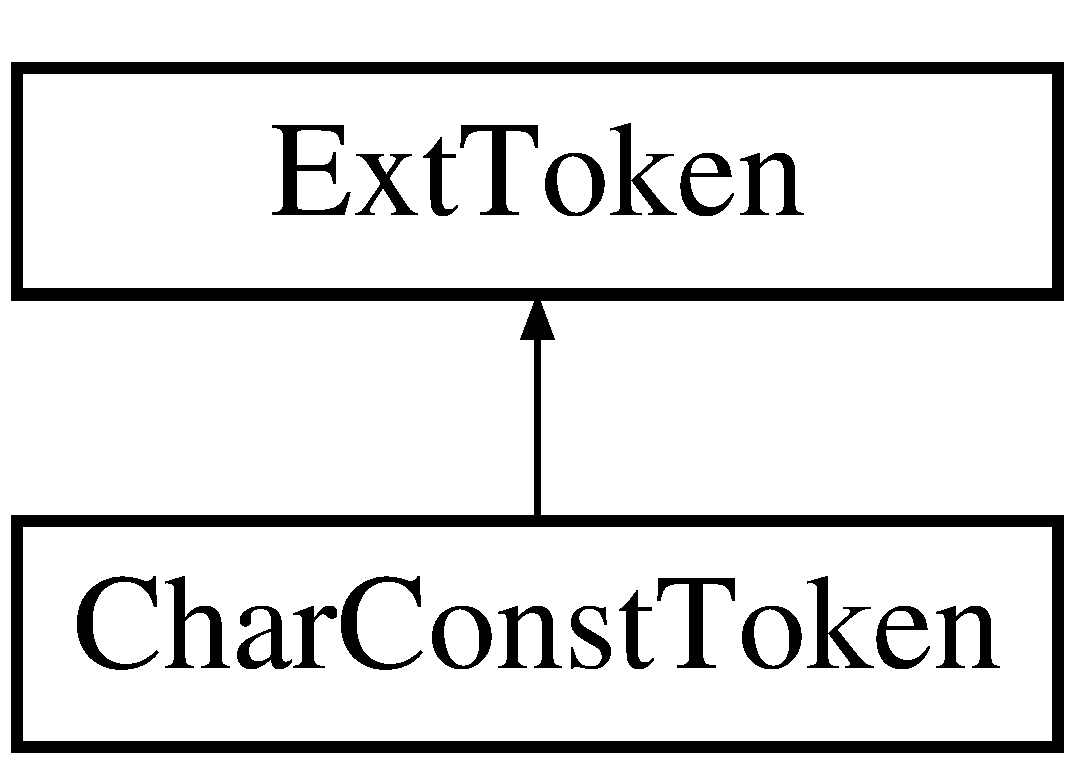
\includegraphics[height=2.000000cm]{class_char_const_token}
\end{center}
\end{figure}
\subsection*{Public Member Functions}
\begin{DoxyCompactItemize}
\item 
\hypertarget{class_char_const_token_a9dcb8d0d26c4f9c66570357641933c51}{}{\bfseries Char\+Const\+Token} (\hyperlink{class_parser}{Parser} $\ast$p, \hyperlink{class_token}{Token} $\ast$t)\label{class_char_const_token_a9dcb8d0d26c4f9c66570357641933c51}

\item 
\hypertarget{class_char_const_token_a33032d6b35ef2b6ebc4db770b374ad5b}{}\hyperlink{class_parse_result}{Parse\+Result} {\bfseries nud} ()\label{class_char_const_token_a33032d6b35ef2b6ebc4db770b374ad5b}

\item 
\hypertarget{class_char_const_token_addf2603d51bc2be908137f06737d8b30}{}std\+::string {\bfseries description} ()\label{class_char_const_token_addf2603d51bc2be908137f06737d8b30}

\end{DoxyCompactItemize}
\subsection*{Additional Inherited Members}


The documentation for this class was generated from the following file\+:\begin{DoxyCompactItemize}
\item 
ext\+Token.\+h\end{DoxyCompactItemize}

\hypertarget{class_dash_token}{}\section{Dash\+Token Class Reference}
\label{class_dash_token}\index{Dash\+Token@{Dash\+Token}}
Inheritance diagram for Dash\+Token\+:\begin{figure}[H]
\begin{center}
\leavevmode
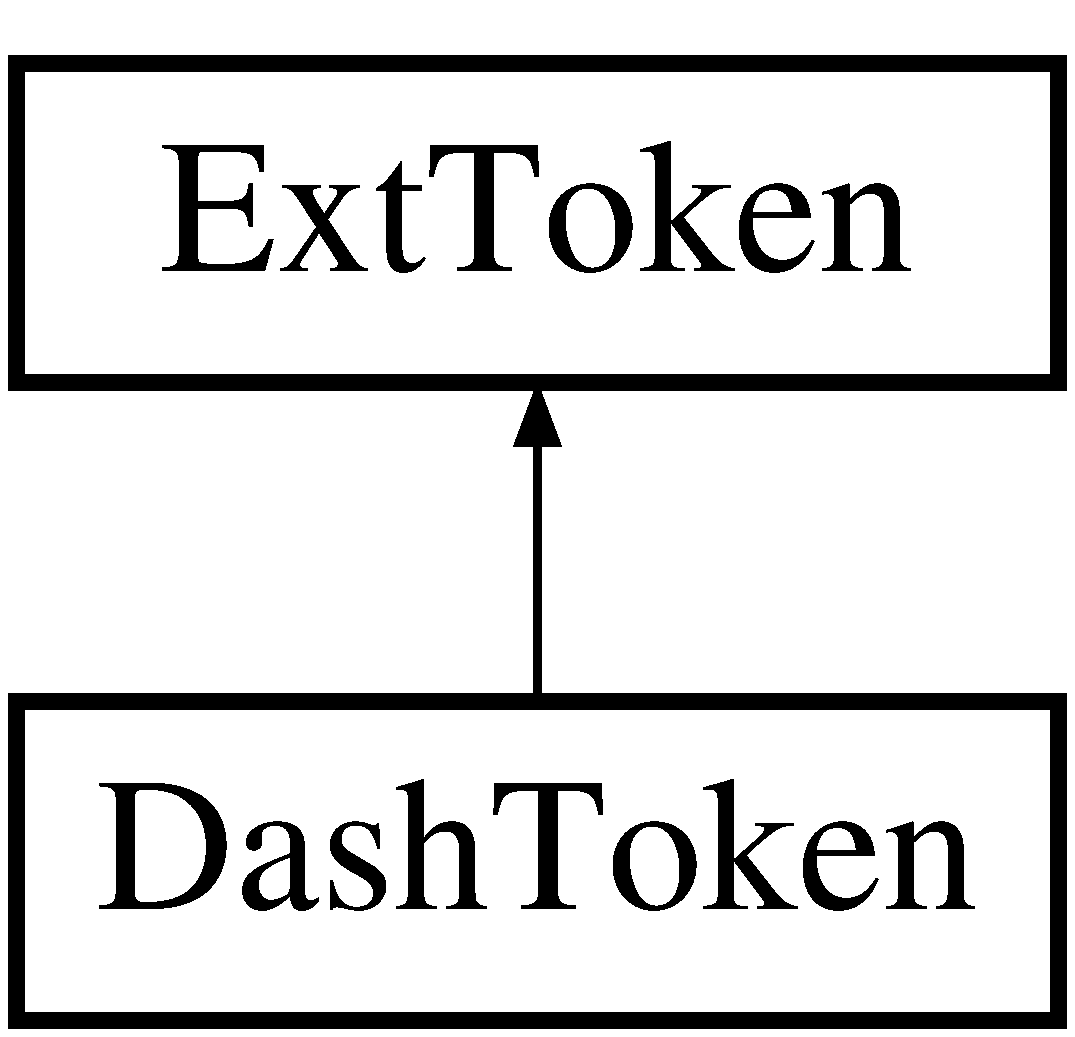
\includegraphics[height=2.000000cm]{class_dash_token}
\end{center}
\end{figure}
\subsection*{Public Member Functions}
\begin{DoxyCompactItemize}
\item 
\hypertarget{class_dash_token_a9570d66563405c728e679b63a44e53e2}{}{\bfseries Dash\+Token} (\hyperlink{class_parser}{Parser} $\ast$p, \hyperlink{class_token}{Token} $\ast$t)\label{class_dash_token_a9570d66563405c728e679b63a44e53e2}

\item 
\hypertarget{class_dash_token_a703ca6afcd05ac4688c66b82e177bdbc}{}\hyperlink{class_parse_result}{Parse\+Result} {\bfseries led} (\hyperlink{class_parse_result}{Parse\+Result} left)\label{class_dash_token_a703ca6afcd05ac4688c66b82e177bdbc}

\item 
\hypertarget{class_dash_token_a02d79abb30dcab20081edb8e969885d2}{}std\+::string {\bfseries description} ()\label{class_dash_token_a02d79abb30dcab20081edb8e969885d2}

\item 
\hypertarget{class_dash_token_a1cf877584a85c06e884a182744e92b39}{}int {\bfseries lbp} ()\label{class_dash_token_a1cf877584a85c06e884a182744e92b39}

\end{DoxyCompactItemize}
\subsection*{Additional Inherited Members}


The documentation for this class was generated from the following file\+:\begin{DoxyCompactItemize}
\item 
ext\+Token.\+h\end{DoxyCompactItemize}

\hypertarget{class_end_of_file_token}{}\section{End\+Of\+File\+Token Class Reference}
\label{class_end_of_file_token}\index{End\+Of\+File\+Token@{End\+Of\+File\+Token}}
Inheritance diagram for End\+Of\+File\+Token\+:\begin{figure}[H]
\begin{center}
\leavevmode
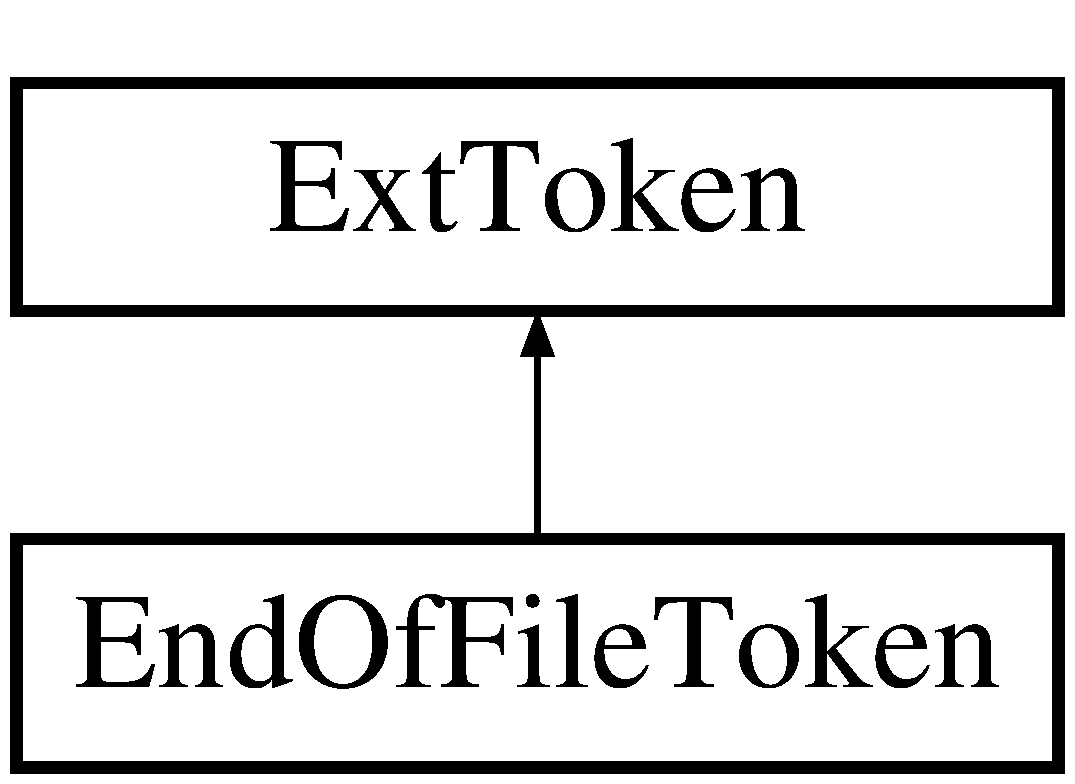
\includegraphics[height=2.000000cm]{class_end_of_file_token}
\end{center}
\end{figure}
\subsection*{Public Member Functions}
\begin{DoxyCompactItemize}
\item 
\hypertarget{class_end_of_file_token_a5c093bc13648a4f4df525ea4242e59d9}{}{\bfseries End\+Of\+File\+Token} (\hyperlink{class_parser}{Parser} $\ast$p, \hyperlink{class_token}{Token} $\ast$t)\label{class_end_of_file_token_a5c093bc13648a4f4df525ea4242e59d9}

\item 
\hypertarget{class_end_of_file_token_a918312b101ca8cc7fb5ba4e56bc12b58}{}std\+::string {\bfseries description} ()\label{class_end_of_file_token_a918312b101ca8cc7fb5ba4e56bc12b58}

\end{DoxyCompactItemize}
\subsection*{Additional Inherited Members}


The documentation for this class was generated from the following file\+:\begin{DoxyCompactItemize}
\item 
ext\+Token.\+h\end{DoxyCompactItemize}

\hypertarget{class_ext_token}{}\section{Ext\+Token Class Reference}
\label{class_ext_token}\index{Ext\+Token@{Ext\+Token}}
Inheritance diagram for Ext\+Token\+:\begin{figure}[H]
\begin{center}
\leavevmode
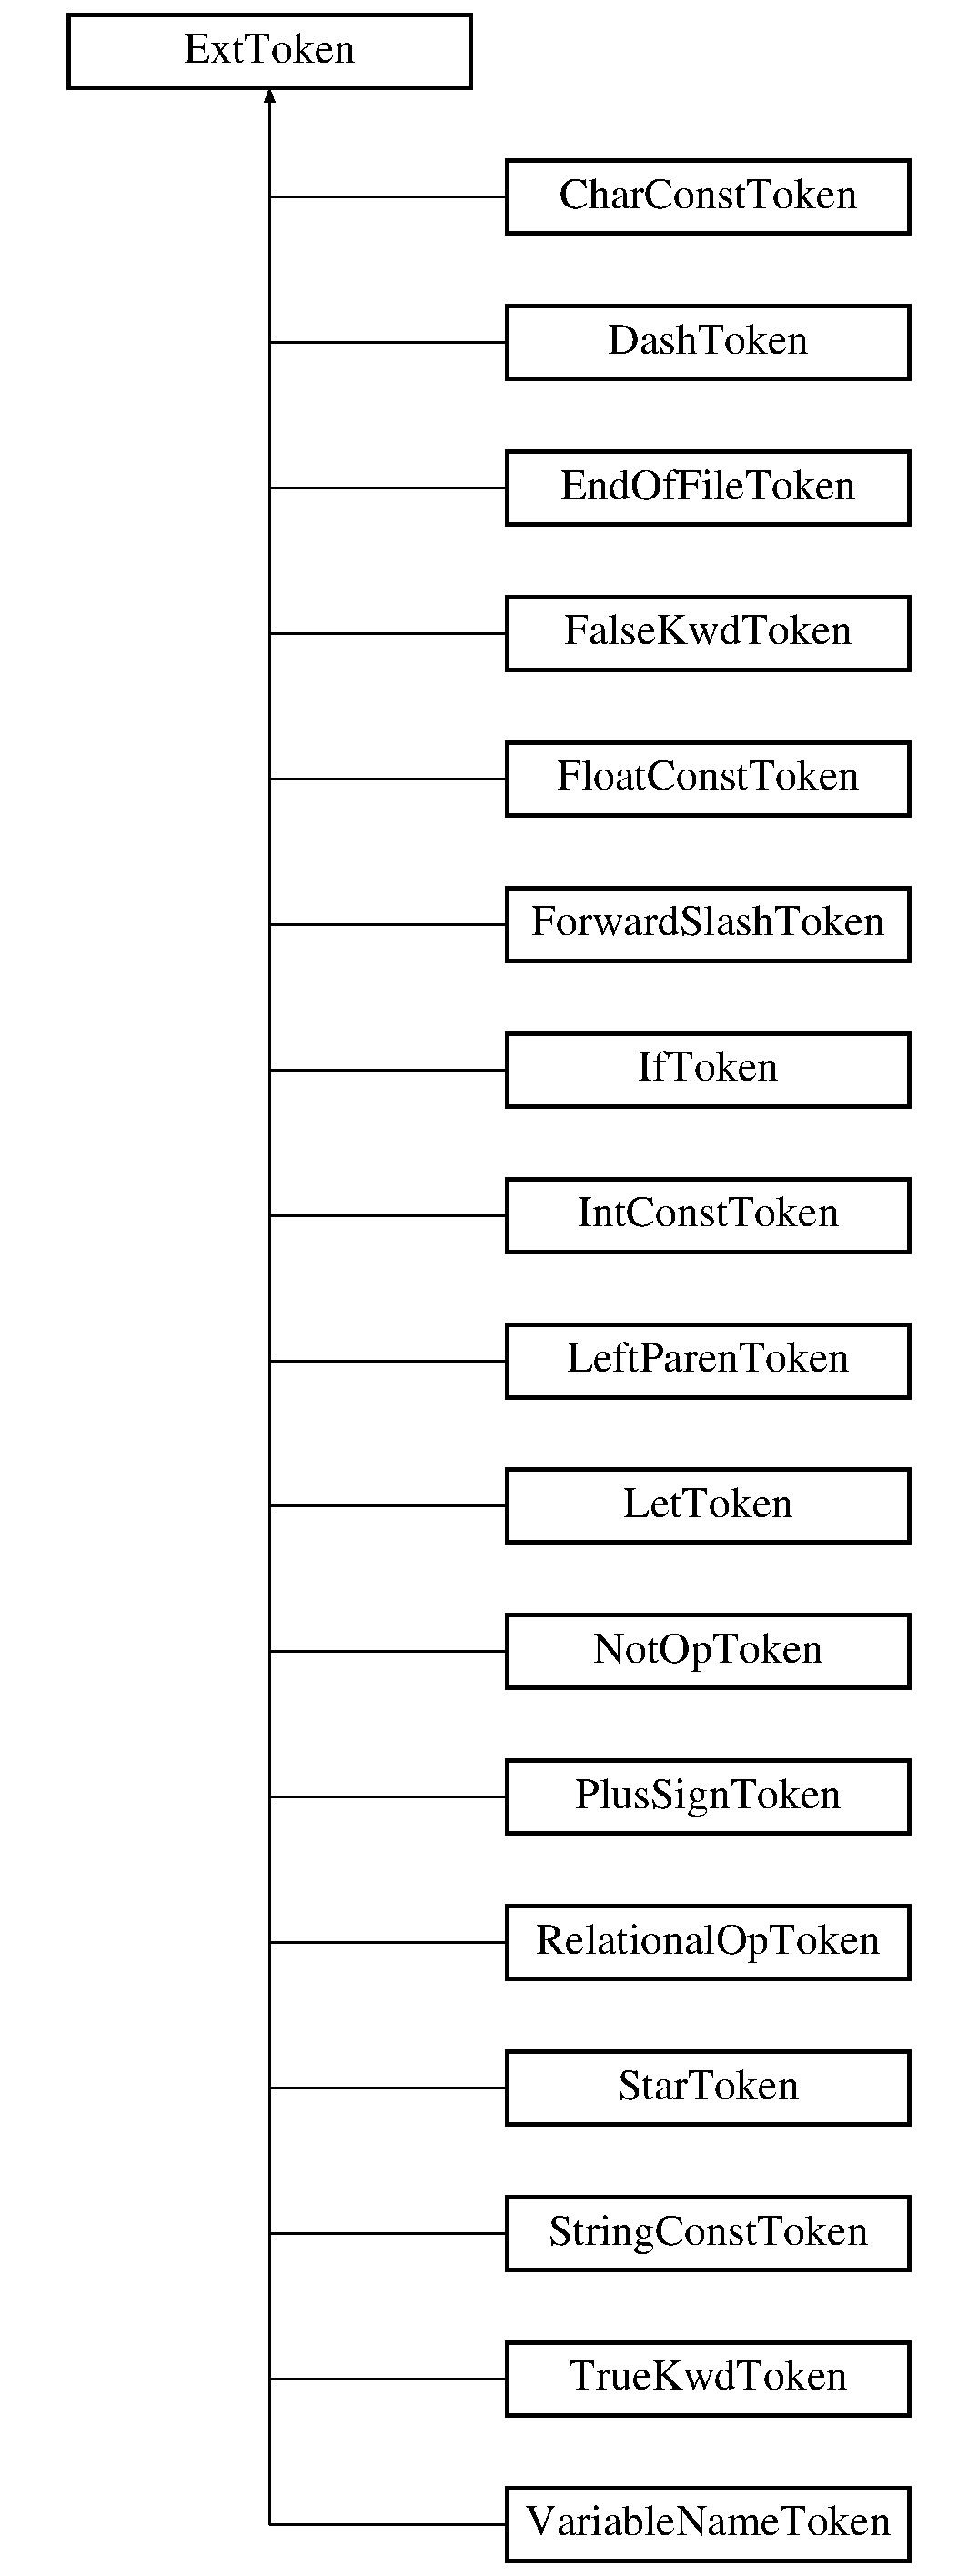
\includegraphics[height=12.000000cm]{class_ext_token}
\end{center}
\end{figure}
\subsection*{Public Member Functions}
\begin{DoxyCompactItemize}
\item 
\hypertarget{class_ext_token_a45a27528f391faf5679b7b30563ce846}{}{\bfseries Ext\+Token} (\hyperlink{class_parser}{Parser} $\ast$p, \hyperlink{class_token}{Token} $\ast$t)\label{class_ext_token_a45a27528f391faf5679b7b30563ce846}

\item 
\hypertarget{class_ext_token_afa8972152abec42cd52b6f6f70a9a179}{}{\bfseries Ext\+Token} (\hyperlink{class_parser}{Parser} $\ast$p, \hyperlink{class_token}{Token} $\ast$t, std\+::string d)\label{class_ext_token_afa8972152abec42cd52b6f6f70a9a179}

\item 
\hypertarget{class_ext_token_a5c21a5ffe91f212085259126652ab77c}{}virtual \hyperlink{class_parse_result}{Parse\+Result} {\bfseries nud} ()\label{class_ext_token_a5c21a5ffe91f212085259126652ab77c}

\item 
\hypertarget{class_ext_token_afb2c9b0040e198d1d8aa2e041c5a7211}{}virtual \hyperlink{class_parse_result}{Parse\+Result} {\bfseries led} (\hyperlink{class_parse_result}{Parse\+Result} left)\label{class_ext_token_afb2c9b0040e198d1d8aa2e041c5a7211}

\item 
\hypertarget{class_ext_token_a6c0d61faa058b71147dd54bacee1db94}{}virtual int {\bfseries lbp} ()\label{class_ext_token_a6c0d61faa058b71147dd54bacee1db94}

\item 
\hypertarget{class_ext_token_a4ab6e72ac23235650b1756f794172ebb}{}virtual std\+::string {\bfseries description} ()\label{class_ext_token_a4ab6e72ac23235650b1756f794172ebb}

\end{DoxyCompactItemize}
\subsection*{Public Attributes}
\begin{DoxyCompactItemize}
\item 
\hypertarget{class_ext_token_a5af1643a542ef7ee8ca0f82706383ae3}{}std\+::string {\bfseries lexeme}\label{class_ext_token_a5af1643a542ef7ee8ca0f82706383ae3}

\item 
\hypertarget{class_ext_token_abbdaef42b65403cdc0247839ef95c875}{}token\+Type {\bfseries terminal}\label{class_ext_token_abbdaef42b65403cdc0247839ef95c875}

\item 
\hypertarget{class_ext_token_aa02995a897183b2a6ef758e541534e46}{}\hyperlink{class_ext_token}{Ext\+Token} $\ast$ {\bfseries next}\label{class_ext_token_aa02995a897183b2a6ef758e541534e46}

\item 
\hypertarget{class_ext_token_af70d22156d5f8e855a8b0d92a82706ba}{}\hyperlink{class_parser}{Parser} $\ast$ {\bfseries parser}\label{class_ext_token_af70d22156d5f8e855a8b0d92a82706ba}

\end{DoxyCompactItemize}


The documentation for this class was generated from the following file\+:\begin{DoxyCompactItemize}
\item 
ext\+Token.\+h\end{DoxyCompactItemize}

\hypertarget{class_false_kwd_token}{}\section{False\+Kwd\+Token Class Reference}
\label{class_false_kwd_token}\index{False\+Kwd\+Token@{False\+Kwd\+Token}}
Inheritance diagram for False\+Kwd\+Token\+:\begin{figure}[H]
\begin{center}
\leavevmode
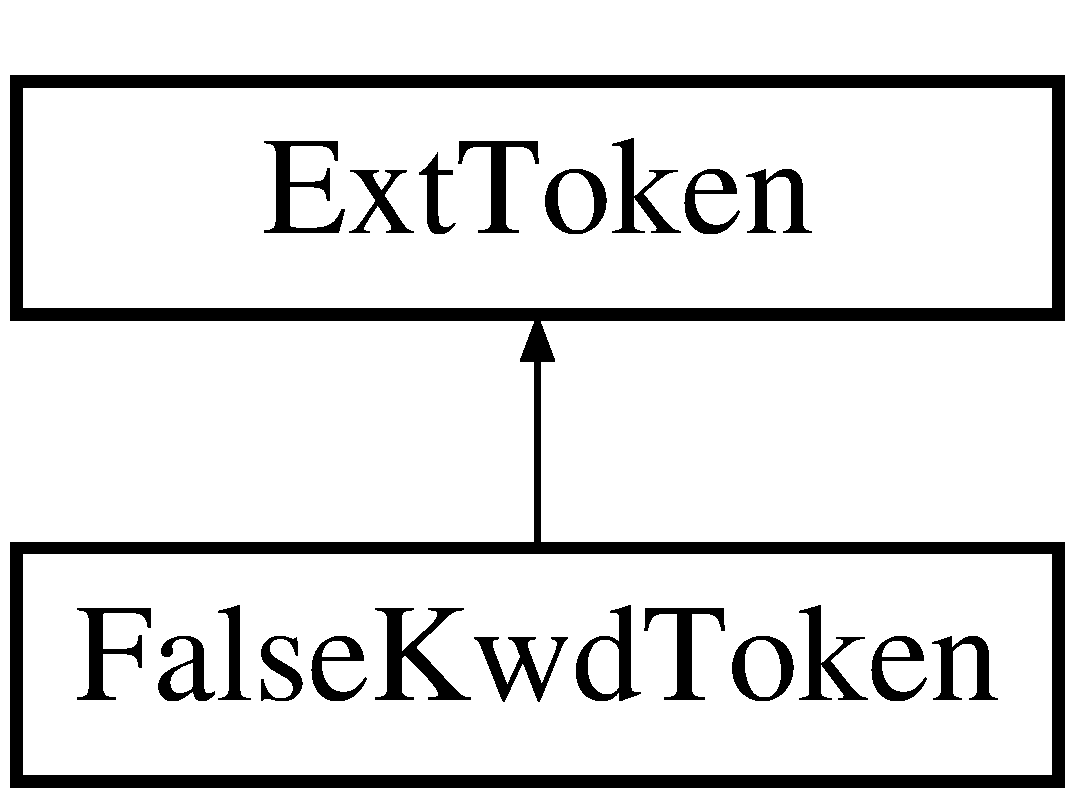
\includegraphics[height=2.000000cm]{class_false_kwd_token}
\end{center}
\end{figure}
\subsection*{Public Member Functions}
\begin{DoxyCompactItemize}
\item 
\hypertarget{class_false_kwd_token_add6402d29fd7b22253a0dc73370597e4}{}{\bfseries False\+Kwd\+Token} (\hyperlink{class_parser}{Parser} $\ast$p, \hyperlink{class_token}{Token} $\ast$t)\label{class_false_kwd_token_add6402d29fd7b22253a0dc73370597e4}

\item 
\hypertarget{class_false_kwd_token_adc06b0433535d552c1e7f8076d756fb3}{}\hyperlink{class_parse_result}{Parse\+Result} {\bfseries nud} ()\label{class_false_kwd_token_adc06b0433535d552c1e7f8076d756fb3}

\item 
\hypertarget{class_false_kwd_token_a8351fad7090214687138e113b5a581f1}{}std\+::string {\bfseries description} ()\label{class_false_kwd_token_a8351fad7090214687138e113b5a581f1}

\end{DoxyCompactItemize}
\subsection*{Additional Inherited Members}


The documentation for this class was generated from the following file\+:\begin{DoxyCompactItemize}
\item 
ext\+Token.\+h\end{DoxyCompactItemize}

\hypertarget{class_float_const_token}{}\section{Float\+Const\+Token Class Reference}
\label{class_float_const_token}\index{Float\+Const\+Token@{Float\+Const\+Token}}
Inheritance diagram for Float\+Const\+Token\+:\begin{figure}[H]
\begin{center}
\leavevmode
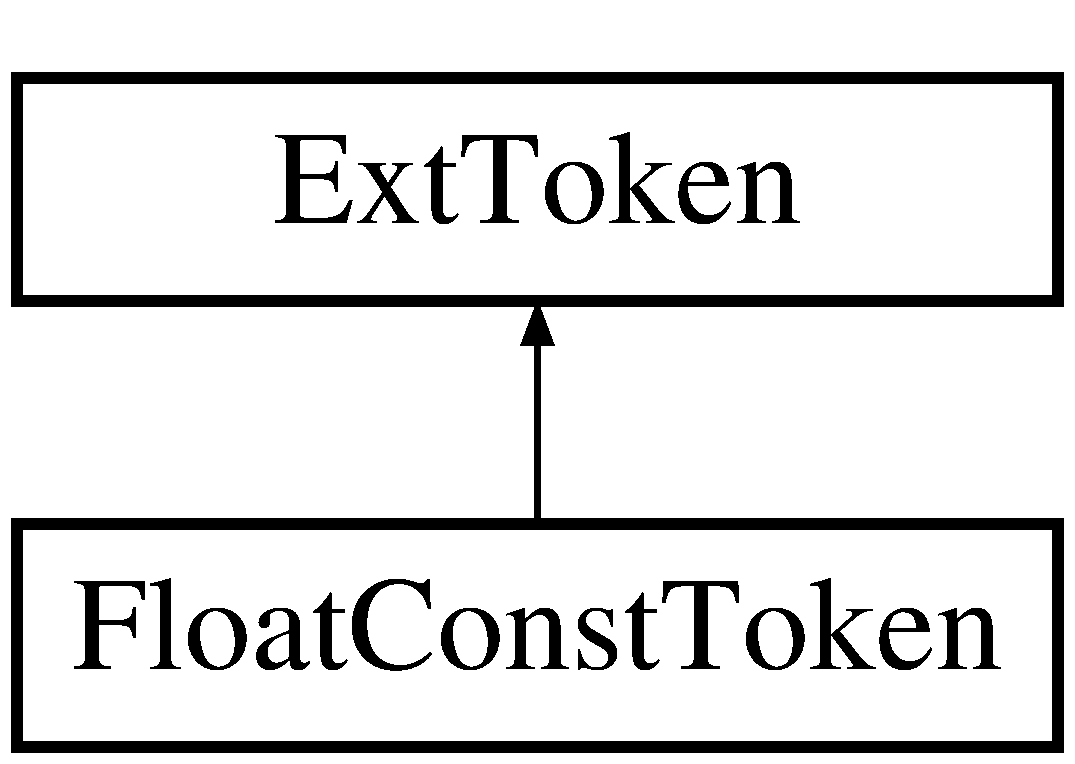
\includegraphics[height=2.000000cm]{class_float_const_token}
\end{center}
\end{figure}
\subsection*{Public Member Functions}
\begin{DoxyCompactItemize}
\item 
\hypertarget{class_float_const_token_aecee1d0e4e8a9410701c68c30858a4db}{}{\bfseries Float\+Const\+Token} (\hyperlink{class_parser}{Parser} $\ast$p, \hyperlink{class_token}{Token} $\ast$t)\label{class_float_const_token_aecee1d0e4e8a9410701c68c30858a4db}

\item 
\hypertarget{class_float_const_token_a991e92ae34d0b01a3b1dd08ed01b8e6e}{}\hyperlink{class_parse_result}{Parse\+Result} {\bfseries nud} ()\label{class_float_const_token_a991e92ae34d0b01a3b1dd08ed01b8e6e}

\item 
\hypertarget{class_float_const_token_a529b6d3ad479b0f6b940a82ba48b98c0}{}std\+::string {\bfseries description} ()\label{class_float_const_token_a529b6d3ad479b0f6b940a82ba48b98c0}

\end{DoxyCompactItemize}
\subsection*{Additional Inherited Members}


The documentation for this class was generated from the following file\+:\begin{DoxyCompactItemize}
\item 
ext\+Token.\+h\end{DoxyCompactItemize}

\hypertarget{class_forward_slash_token}{}\section{Forward\+Slash\+Token Class Reference}
\label{class_forward_slash_token}\index{Forward\+Slash\+Token@{Forward\+Slash\+Token}}
Inheritance diagram for Forward\+Slash\+Token\+:\begin{figure}[H]
\begin{center}
\leavevmode
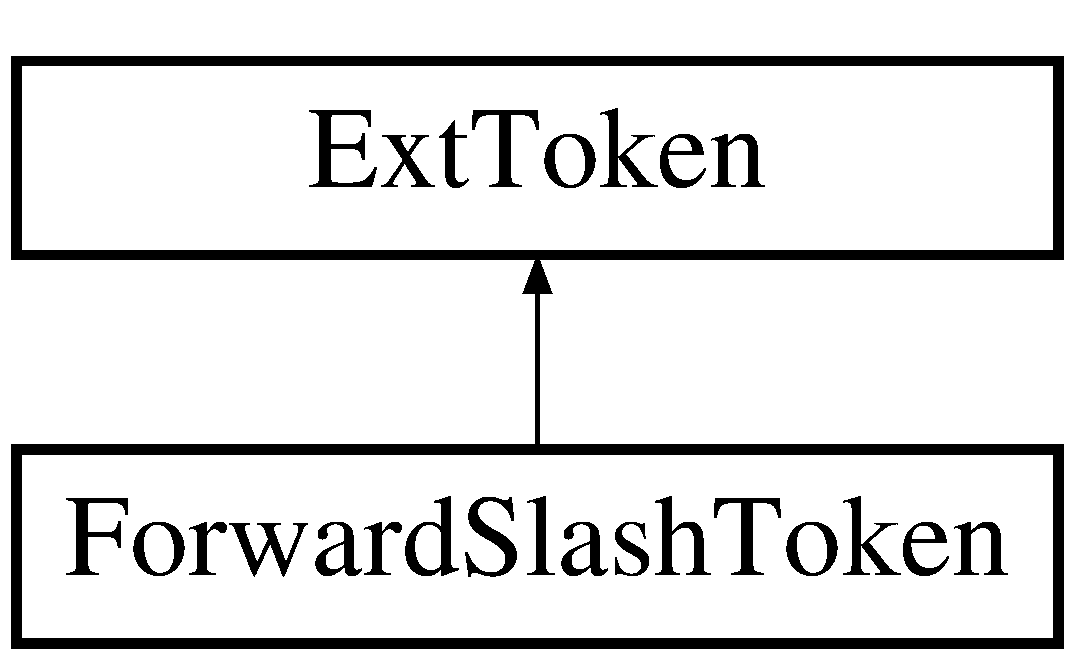
\includegraphics[height=2.000000cm]{class_forward_slash_token}
\end{center}
\end{figure}
\subsection*{Public Member Functions}
\begin{DoxyCompactItemize}
\item 
\hypertarget{class_forward_slash_token_ae818840269cd15f6f6b00929fb4eb979}{}{\bfseries Forward\+Slash\+Token} (\hyperlink{class_parser}{Parser} $\ast$p, \hyperlink{class_token}{Token} $\ast$t)\label{class_forward_slash_token_ae818840269cd15f6f6b00929fb4eb979}

\item 
\hypertarget{class_forward_slash_token_ac2dda7b791ab555e4323f17baaf323e1}{}\hyperlink{class_parse_result}{Parse\+Result} {\bfseries led} (\hyperlink{class_parse_result}{Parse\+Result} left)\label{class_forward_slash_token_ac2dda7b791ab555e4323f17baaf323e1}

\item 
\hypertarget{class_forward_slash_token_ac27b1ab175ec08c468bd0d4c41636a5c}{}std\+::string {\bfseries description} ()\label{class_forward_slash_token_ac27b1ab175ec08c468bd0d4c41636a5c}

\item 
\hypertarget{class_forward_slash_token_ad65829044355922a291dfbfd3052b183}{}int {\bfseries lbp} ()\label{class_forward_slash_token_ad65829044355922a291dfbfd3052b183}

\end{DoxyCompactItemize}
\subsection*{Additional Inherited Members}


The documentation for this class was generated from the following file\+:\begin{DoxyCompactItemize}
\item 
ext\+Token.\+h\end{DoxyCompactItemize}

\hypertarget{class_if_token}{}\section{If\+Token Class Reference}
\label{class_if_token}\index{If\+Token@{If\+Token}}
Inheritance diagram for If\+Token\+:\begin{figure}[H]
\begin{center}
\leavevmode
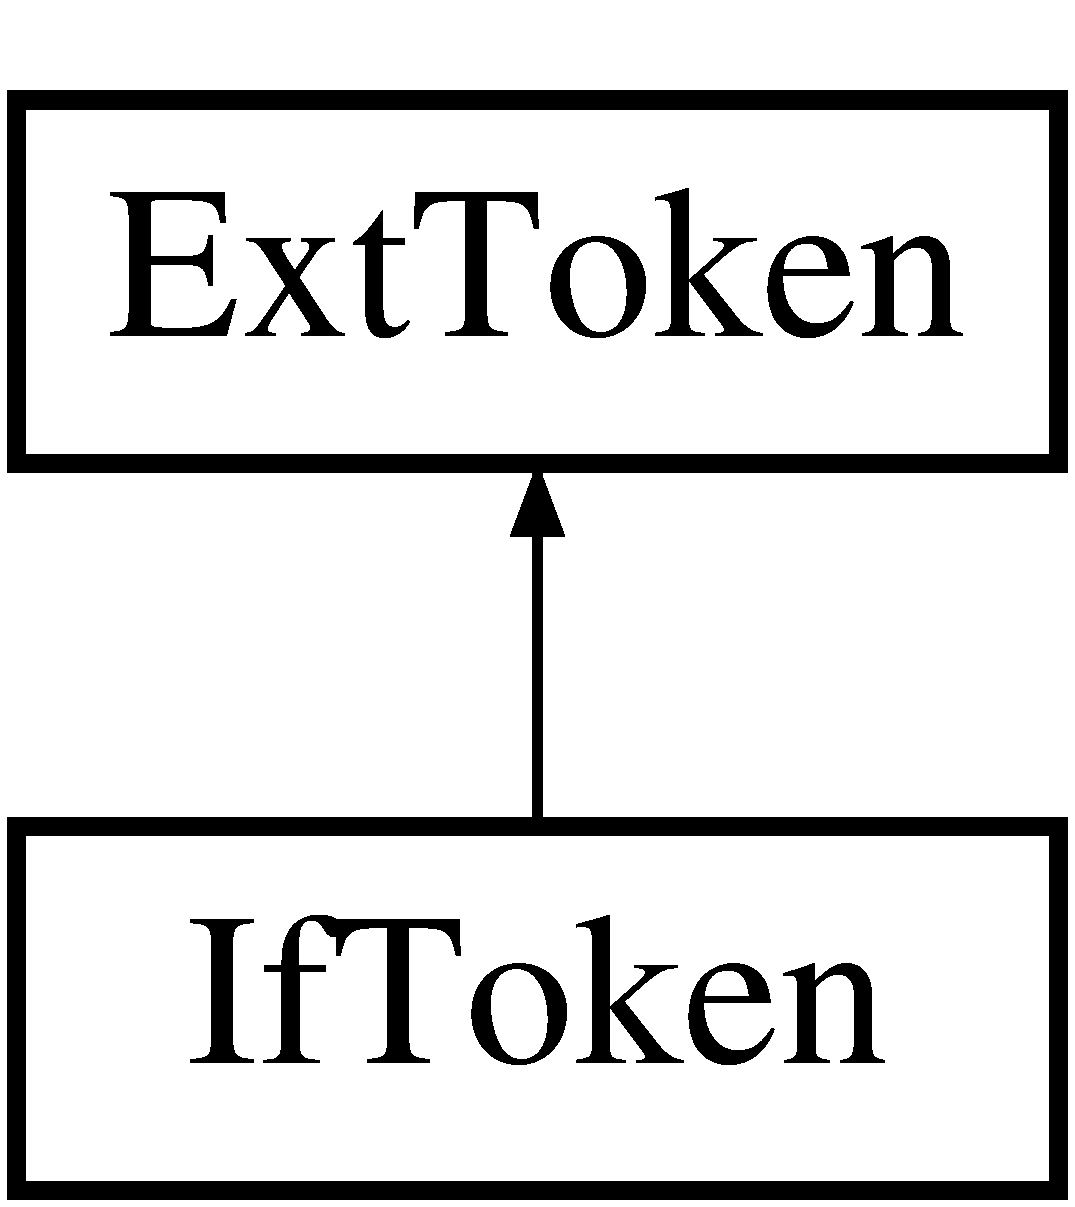
\includegraphics[height=2.000000cm]{class_if_token}
\end{center}
\end{figure}
\subsection*{Public Member Functions}
\begin{DoxyCompactItemize}
\item 
\hypertarget{class_if_token_a607028595b06b8a950000ba3e82329db}{}{\bfseries If\+Token} (\hyperlink{class_parser}{Parser} $\ast$p, \hyperlink{class_token}{Token} $\ast$t)\label{class_if_token_a607028595b06b8a950000ba3e82329db}

\item 
\hypertarget{class_if_token_add06bd79ce755fd5503f78e507109e52}{}\hyperlink{class_parse_result}{Parse\+Result} {\bfseries nud} ()\label{class_if_token_add06bd79ce755fd5503f78e507109e52}

\item 
\hypertarget{class_if_token_aad226162c5649920c13c2a9e9e7a3617}{}std\+::string {\bfseries description} ()\label{class_if_token_aad226162c5649920c13c2a9e9e7a3617}

\item 
\hypertarget{class_if_token_abfd39ff4c4818d382bf0b97fd097c478}{}int {\bfseries lbp} ()\label{class_if_token_abfd39ff4c4818d382bf0b97fd097c478}

\end{DoxyCompactItemize}
\subsection*{Additional Inherited Members}


The documentation for this class was generated from the following file\+:\begin{DoxyCompactItemize}
\item 
ext\+Token.\+h\end{DoxyCompactItemize}

\hypertarget{class_int_const_token}{}\section{Int\+Const\+Token Class Reference}
\label{class_int_const_token}\index{Int\+Const\+Token@{Int\+Const\+Token}}
Inheritance diagram for Int\+Const\+Token\+:\begin{figure}[H]
\begin{center}
\leavevmode
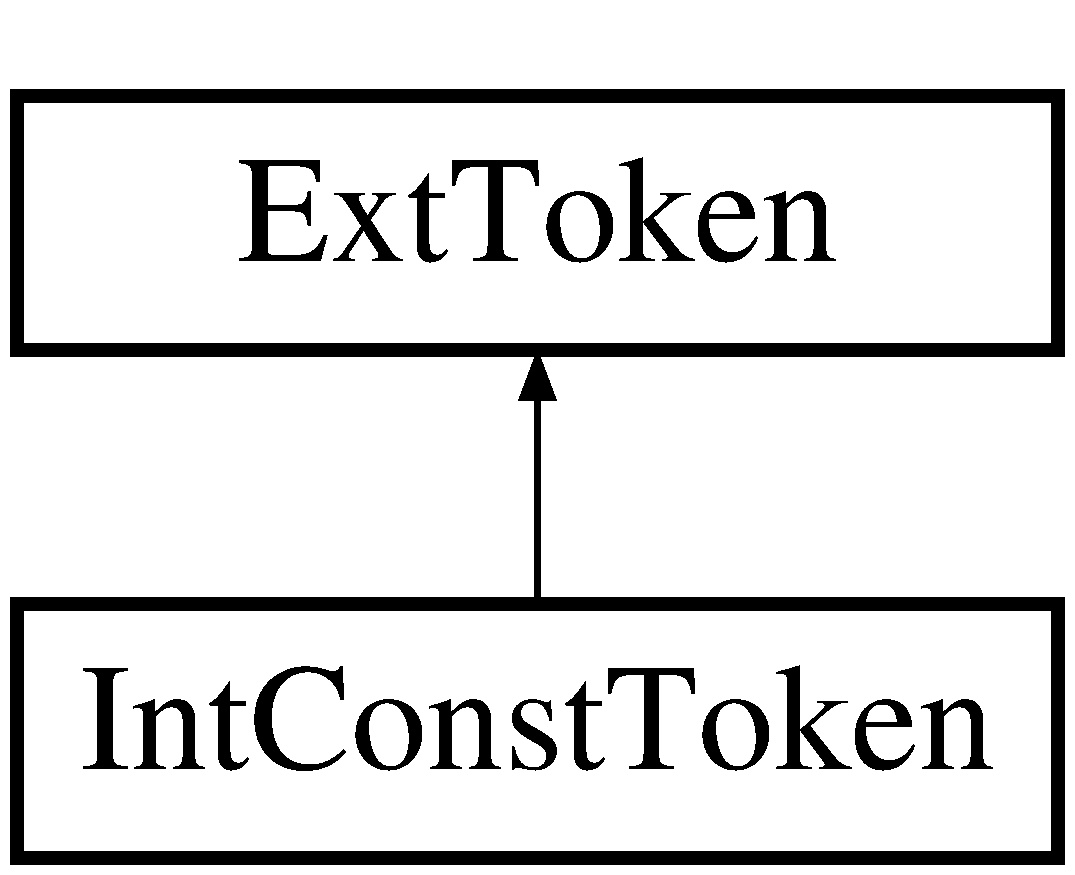
\includegraphics[height=2.000000cm]{class_int_const_token}
\end{center}
\end{figure}
\subsection*{Public Member Functions}
\begin{DoxyCompactItemize}
\item 
\hypertarget{class_int_const_token_a14c6bf0af5a915969b4fef1758067af3}{}{\bfseries Int\+Const\+Token} (\hyperlink{class_parser}{Parser} $\ast$p, \hyperlink{class_token}{Token} $\ast$t)\label{class_int_const_token_a14c6bf0af5a915969b4fef1758067af3}

\item 
\hypertarget{class_int_const_token_ae1f720d6006c47e145cae7879d09c708}{}\hyperlink{class_parse_result}{Parse\+Result} {\bfseries nud} ()\label{class_int_const_token_ae1f720d6006c47e145cae7879d09c708}

\item 
\hypertarget{class_int_const_token_a98191508d849878d40800e447a0f1892}{}std\+::string {\bfseries description} ()\label{class_int_const_token_a98191508d849878d40800e447a0f1892}

\end{DoxyCompactItemize}
\subsection*{Additional Inherited Members}


The documentation for this class was generated from the following file\+:\begin{DoxyCompactItemize}
\item 
ext\+Token.\+h\end{DoxyCompactItemize}

\hypertarget{class_left_paren_token}{}\section{Left\+Paren\+Token Class Reference}
\label{class_left_paren_token}\index{Left\+Paren\+Token@{Left\+Paren\+Token}}
Inheritance diagram for Left\+Paren\+Token\+:\begin{figure}[H]
\begin{center}
\leavevmode
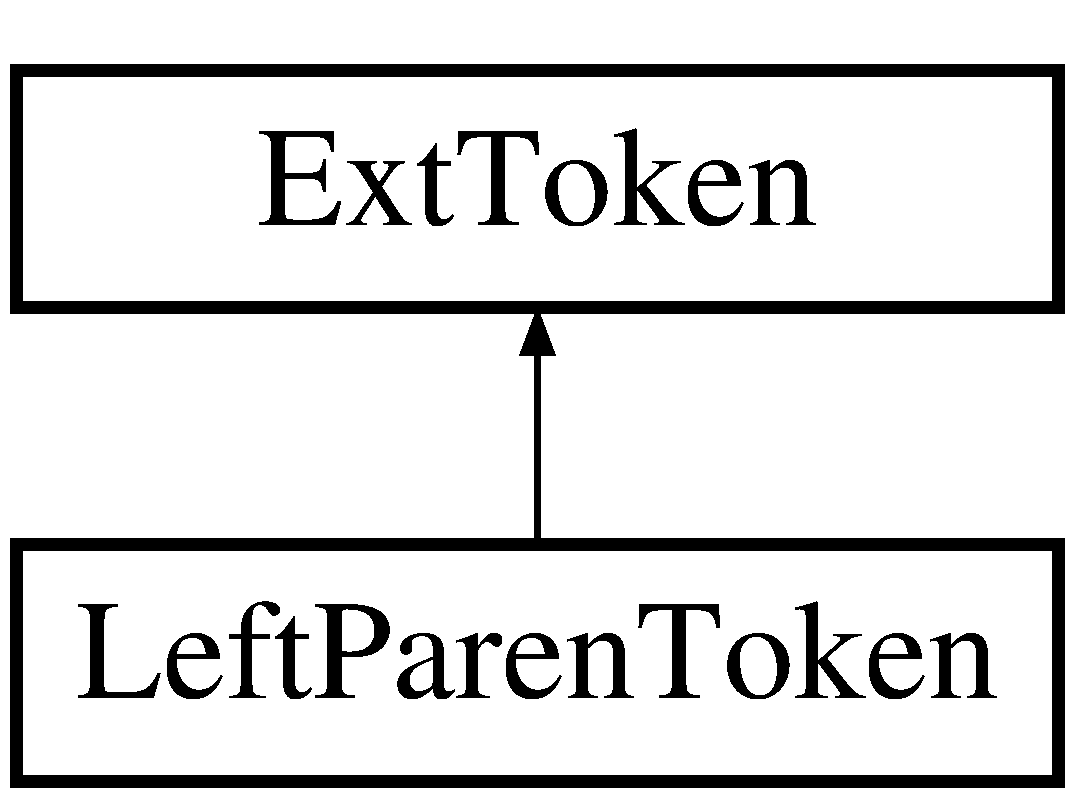
\includegraphics[height=2.000000cm]{class_left_paren_token}
\end{center}
\end{figure}
\subsection*{Public Member Functions}
\begin{DoxyCompactItemize}
\item 
\hypertarget{class_left_paren_token_aecdc6faf48a1a7192ec55712f0264cba}{}{\bfseries Left\+Paren\+Token} (\hyperlink{class_parser}{Parser} $\ast$p, \hyperlink{class_token}{Token} $\ast$t)\label{class_left_paren_token_aecdc6faf48a1a7192ec55712f0264cba}

\item 
\hypertarget{class_left_paren_token_a3cb3ae9ab2647e5534c85529d314f08b}{}\hyperlink{class_parse_result}{Parse\+Result} {\bfseries nud} ()\label{class_left_paren_token_a3cb3ae9ab2647e5534c85529d314f08b}

\item 
\hypertarget{class_left_paren_token_a2df35684bd2081c3bdfe2357946917bc}{}std\+::string {\bfseries description} ()\label{class_left_paren_token_a2df35684bd2081c3bdfe2357946917bc}

\item 
\hypertarget{class_left_paren_token_afa1b94645278f097bb097d3b24445d14}{}int {\bfseries lbp} ()\label{class_left_paren_token_afa1b94645278f097bb097d3b24445d14}

\end{DoxyCompactItemize}
\subsection*{Additional Inherited Members}


The documentation for this class was generated from the following file\+:\begin{DoxyCompactItemize}
\item 
ext\+Token.\+h\end{DoxyCompactItemize}

\hypertarget{class_let_token}{}\section{Let\+Token Class Reference}
\label{class_let_token}\index{Let\+Token@{Let\+Token}}
Inheritance diagram for Let\+Token\+:\begin{figure}[H]
\begin{center}
\leavevmode
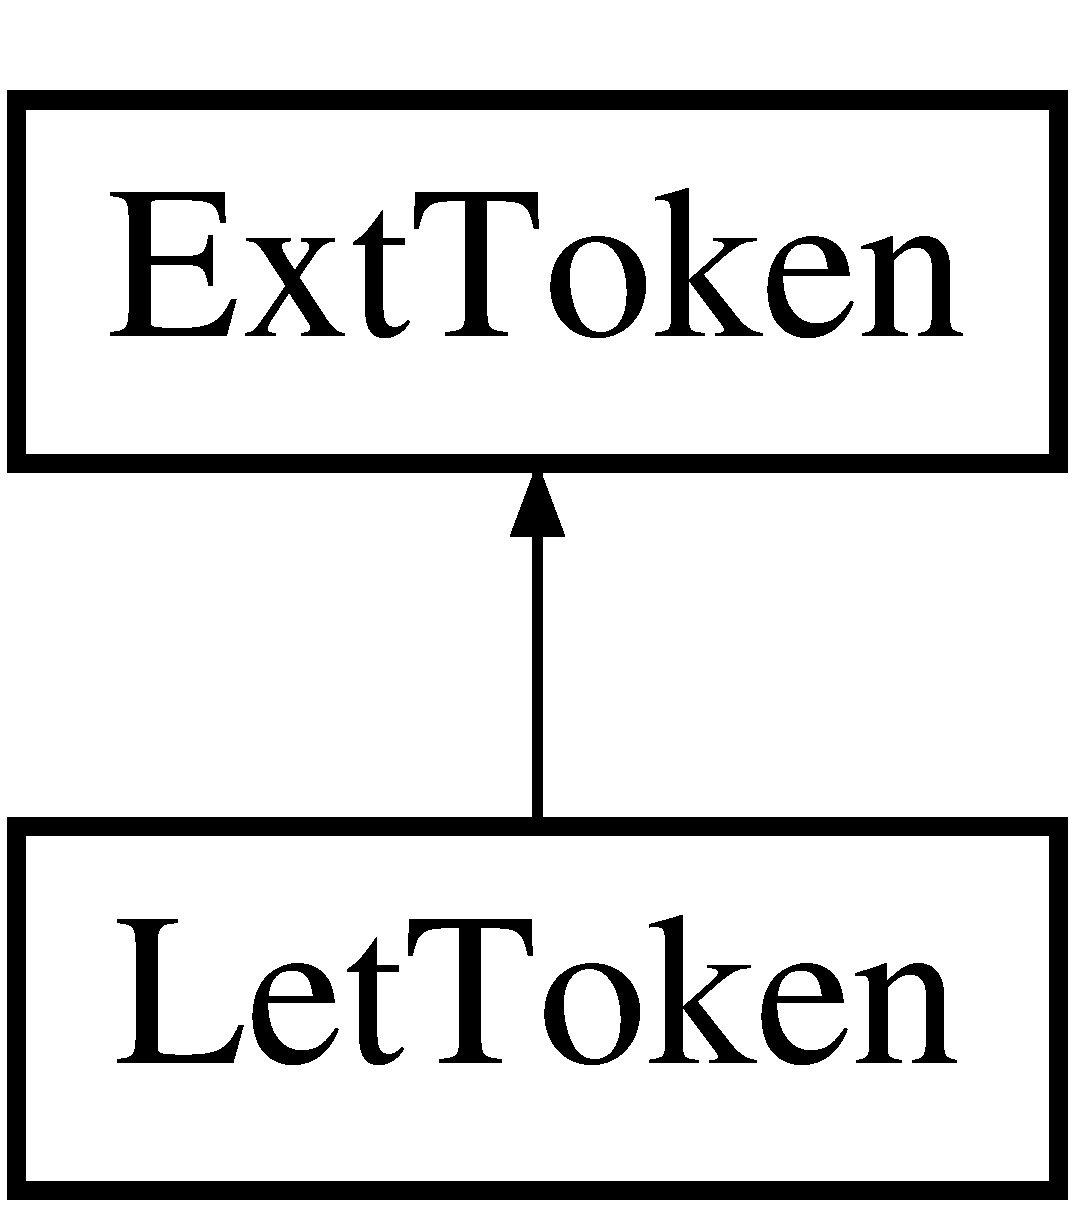
\includegraphics[height=2.000000cm]{class_let_token}
\end{center}
\end{figure}
\subsection*{Public Member Functions}
\begin{DoxyCompactItemize}
\item 
\hypertarget{class_let_token_a94651a82207e47cd2c1066a58cb1fe08}{}{\bfseries Let\+Token} (\hyperlink{class_parser}{Parser} $\ast$p, \hyperlink{class_token}{Token} $\ast$t)\label{class_let_token_a94651a82207e47cd2c1066a58cb1fe08}

\item 
\hypertarget{class_let_token_a14df948cdf775bde8392bf58d53b91f3}{}\hyperlink{class_parse_result}{Parse\+Result} {\bfseries nud} ()\label{class_let_token_a14df948cdf775bde8392bf58d53b91f3}

\item 
\hypertarget{class_let_token_a2c5ba0489774bf6468a26f4e19d7fab4}{}std\+::string {\bfseries description} ()\label{class_let_token_a2c5ba0489774bf6468a26f4e19d7fab4}

\item 
\hypertarget{class_let_token_a2a5ab5bc5897340513480c162bb2b065}{}int {\bfseries lbp} ()\label{class_let_token_a2a5ab5bc5897340513480c162bb2b065}

\end{DoxyCompactItemize}
\subsection*{Additional Inherited Members}


The documentation for this class was generated from the following file\+:\begin{DoxyCompactItemize}
\item 
ext\+Token.\+h\end{DoxyCompactItemize}

\hypertarget{class_not_op_token}{}\section{Not\+Op\+Token Class Reference}
\label{class_not_op_token}\index{Not\+Op\+Token@{Not\+Op\+Token}}
Inheritance diagram for Not\+Op\+Token\+:\begin{figure}[H]
\begin{center}
\leavevmode
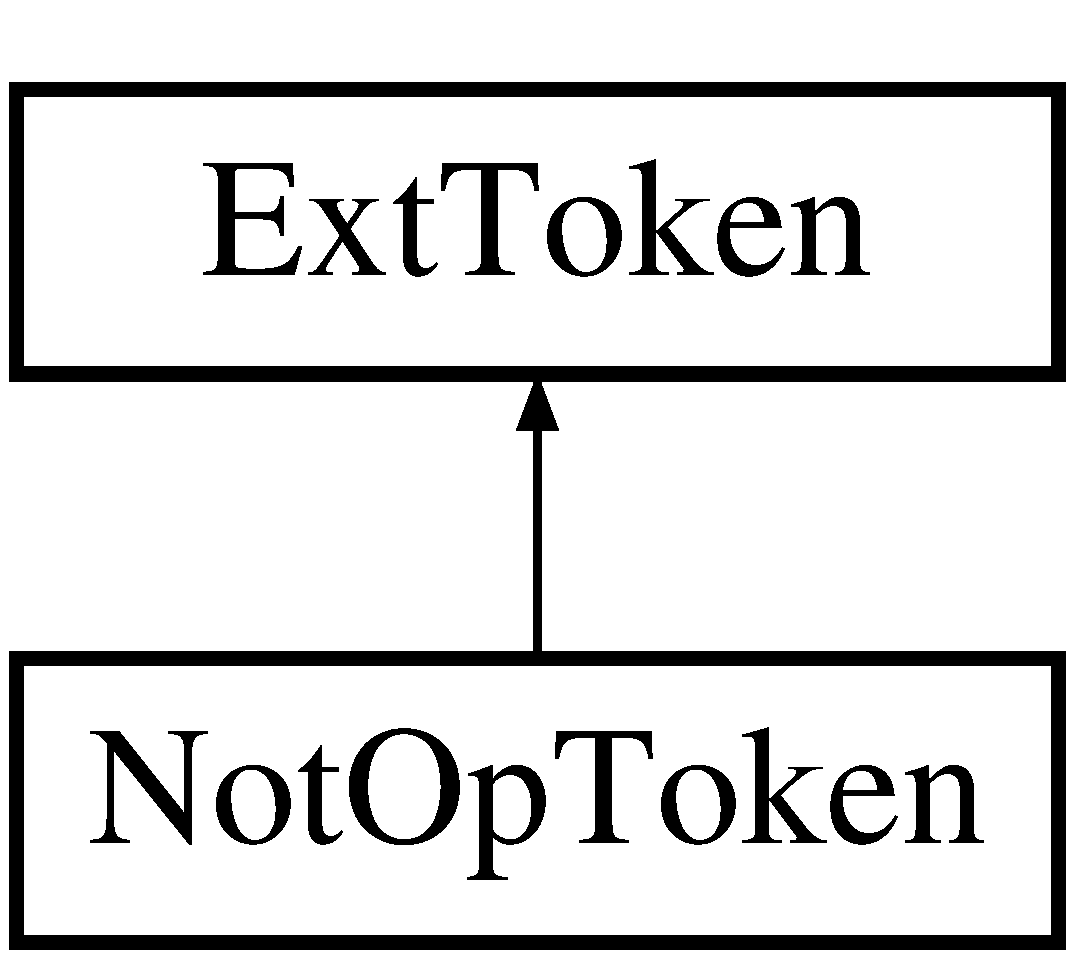
\includegraphics[height=2.000000cm]{class_not_op_token}
\end{center}
\end{figure}
\subsection*{Public Member Functions}
\begin{DoxyCompactItemize}
\item 
\hypertarget{class_not_op_token_afb8b9e96a178b1dfd69abf0a901dfddf}{}{\bfseries Not\+Op\+Token} (\hyperlink{class_parser}{Parser} $\ast$p, \hyperlink{class_token}{Token} $\ast$t)\label{class_not_op_token_afb8b9e96a178b1dfd69abf0a901dfddf}

\item 
\hypertarget{class_not_op_token_a55a0dd53742aaca04338c16be079b031}{}\hyperlink{class_parse_result}{Parse\+Result} {\bfseries nud} ()\label{class_not_op_token_a55a0dd53742aaca04338c16be079b031}

\item 
\hypertarget{class_not_op_token_a136a11f1e42542a9a58b7c14249c9d23}{}std\+::string {\bfseries description} ()\label{class_not_op_token_a136a11f1e42542a9a58b7c14249c9d23}

\end{DoxyCompactItemize}
\subsection*{Additional Inherited Members}


The documentation for this class was generated from the following file\+:\begin{DoxyCompactItemize}
\item 
ext\+Token.\+h\end{DoxyCompactItemize}

\hypertarget{class_parser}{}\section{Parser Class Reference}
\label{class_parser}\index{Parser@{Parser}}
\subsection*{Public Member Functions}
\begin{DoxyCompactItemize}
\item 
\hypertarget{class_parser_a2c1a7aa0b09a43bc1eef460817efb1d6}{}\hyperlink{class_parse_result}{Parse\+Result} {\bfseries parse} (const char $\ast$text)\label{class_parser_a2c1a7aa0b09a43bc1eef460817efb1d6}

\item 
\hypertarget{class_parser_a14e25c84322809e2f060dc530362ea71}{}\hyperlink{class_parse_result}{Parse\+Result} {\bfseries parse\+Program} ()\label{class_parser_a14e25c84322809e2f060dc530362ea71}

\item 
\hypertarget{class_parser_ac646227983887c1cd13dae67fa1bc142}{}\hyperlink{class_parse_result}{Parse\+Result} {\bfseries parse\+Decl} ()\label{class_parser_ac646227983887c1cd13dae67fa1bc142}

\item 
\hypertarget{class_parser_a1e1f83c0f4b11148a356d951f191425e}{}\hyperlink{class_parse_result}{Parse\+Result} {\bfseries parse\+Standard\+Decl} ()\label{class_parser_a1e1f83c0f4b11148a356d951f191425e}

\item 
\hypertarget{class_parser_a3a00df25fda2af308b69f05eed14ac69}{}\hyperlink{class_parse_result}{Parse\+Result} {\bfseries parse\+Matrix\+Decl} ()\label{class_parser_a3a00df25fda2af308b69f05eed14ac69}

\item 
\hypertarget{class_parser_a452db3def31683cb0305e57a01489bd4}{}\hyperlink{class_parse_result}{Parse\+Result} {\bfseries parse\+Stmts} ()\label{class_parser_a452db3def31683cb0305e57a01489bd4}

\item 
\hypertarget{class_parser_a9709c4793d0cce012d595f3ee416cd25}{}\hyperlink{class_parse_result}{Parse\+Result} {\bfseries parse\+Stmt} ()\label{class_parser_a9709c4793d0cce012d595f3ee416cd25}

\item 
\hypertarget{class_parser_a50227dc24dc7a175ac0533d9957dfcf8}{}\hyperlink{class_parse_result}{Parse\+Result} {\bfseries parse\+Expr} (int rbp)\label{class_parser_a50227dc24dc7a175ac0533d9957dfcf8}

\item 
\hypertarget{class_parser_ad40f1e5e4c66814f959d982f94b767a3}{}\hyperlink{class_parse_result}{Parse\+Result} {\bfseries parse\+True\+Kwd} ()\label{class_parser_ad40f1e5e4c66814f959d982f94b767a3}

\item 
\hypertarget{class_parser_a56f03d2e70d12648c55ce56a11e63324}{}\hyperlink{class_parse_result}{Parse\+Result} {\bfseries parse\+False\+Kwd} ()\label{class_parser_a56f03d2e70d12648c55ce56a11e63324}

\item 
\hypertarget{class_parser_a2b200b744e5bedf82ef6f610d7877cfc}{}\hyperlink{class_parse_result}{Parse\+Result} {\bfseries parse\+Int\+Const} ()\label{class_parser_a2b200b744e5bedf82ef6f610d7877cfc}

\item 
\hypertarget{class_parser_aaf7b1176fd53246f59577c7eec8b9d22}{}\hyperlink{class_parse_result}{Parse\+Result} {\bfseries parse\+Float\+Const} ()\label{class_parser_aaf7b1176fd53246f59577c7eec8b9d22}

\item 
\hypertarget{class_parser_a4d8930d45c2b730912154c46cc54833c}{}\hyperlink{class_parse_result}{Parse\+Result} {\bfseries parse\+String\+Const} ()\label{class_parser_a4d8930d45c2b730912154c46cc54833c}

\item 
\hypertarget{class_parser_a49c9b3d31ca060c97873e5485d518da3}{}\hyperlink{class_parse_result}{Parse\+Result} {\bfseries parse\+Char\+Const} ()\label{class_parser_a49c9b3d31ca060c97873e5485d518da3}

\item 
\hypertarget{class_parser_a8c1baf62f71da64590e883e51ce622ca}{}\hyperlink{class_parse_result}{Parse\+Result} {\bfseries parse\+Variable\+Name} ()\label{class_parser_a8c1baf62f71da64590e883e51ce622ca}

\item 
\hypertarget{class_parser_aec4c38e1e63c9becfd3a8fc4a1a73f01}{}\hyperlink{class_parse_result}{Parse\+Result} {\bfseries parse\+Nested\+Expr} ()\label{class_parser_aec4c38e1e63c9becfd3a8fc4a1a73f01}

\item 
\hypertarget{class_parser_a1503ceff46112d6d4f0e01b5fb77afcd}{}\hyperlink{class_parse_result}{Parse\+Result} {\bfseries parse\+Not\+Expr} ()\label{class_parser_a1503ceff46112d6d4f0e01b5fb77afcd}

\item 
\hypertarget{class_parser_aa24c33b04779801b330d7fe5a74349e5}{}\hyperlink{class_parse_result}{Parse\+Result} {\bfseries parse\+Let\+Expr} ()\label{class_parser_aa24c33b04779801b330d7fe5a74349e5}

\item 
\hypertarget{class_parser_a555bc6f671d408208e6d049f8e9f3c86}{}\hyperlink{class_parse_result}{Parse\+Result} {\bfseries parse\+If\+Expr} ()\label{class_parser_a555bc6f671d408208e6d049f8e9f3c86}

\item 
\hypertarget{class_parser_ae09cb2b5a7f80c6ad4ad9ccf27a746ca}{}\hyperlink{class_parse_result}{Parse\+Result} {\bfseries parse\+Addition} (\hyperlink{class_parse_result}{Parse\+Result} left)\label{class_parser_ae09cb2b5a7f80c6ad4ad9ccf27a746ca}

\item 
\hypertarget{class_parser_a52e6a57d53fc98e5819cc51b3cbe5bd5}{}\hyperlink{class_parse_result}{Parse\+Result} {\bfseries parse\+Multiplication} (\hyperlink{class_parse_result}{Parse\+Result} left)\label{class_parser_a52e6a57d53fc98e5819cc51b3cbe5bd5}

\item 
\hypertarget{class_parser_ac22cf1f77e0ca4c23942d5cbcc47eb37}{}\hyperlink{class_parse_result}{Parse\+Result} {\bfseries parse\+Subtraction} (\hyperlink{class_parse_result}{Parse\+Result} left)\label{class_parser_ac22cf1f77e0ca4c23942d5cbcc47eb37}

\item 
\hypertarget{class_parser_ad05e6cd1bf83179ecb727b83cbbd0c4e}{}\hyperlink{class_parse_result}{Parse\+Result} {\bfseries parse\+Division} (\hyperlink{class_parse_result}{Parse\+Result} left)\label{class_parser_ad05e6cd1bf83179ecb727b83cbbd0c4e}

\item 
\hypertarget{class_parser_ab42ecabc4dbe601d5ed9667351c0c0b8}{}\hyperlink{class_parse_result}{Parse\+Result} {\bfseries parse\+Relational\+Expr} (\hyperlink{class_parse_result}{Parse\+Result} left)\label{class_parser_ab42ecabc4dbe601d5ed9667351c0c0b8}

\item 
\hypertarget{class_parser_a3199aab5275c8b6477245eb866fabf35}{}void {\bfseries match} (token\+Type tt)\label{class_parser_a3199aab5275c8b6477245eb866fabf35}

\item 
\hypertarget{class_parser_a151ffb920a67527813d77bc4ba44c4a7}{}bool {\bfseries attempt\+Match} (token\+Type tt)\label{class_parser_a151ffb920a67527813d77bc4ba44c4a7}

\item 
\hypertarget{class_parser_a67a10b685bd263477b5f59f1923cdec3}{}bool {\bfseries next\+Is} (token\+Type tt)\label{class_parser_a67a10b685bd263477b5f59f1923cdec3}

\item 
\hypertarget{class_parser_a324a5bb61c9dfc645300a92aecd6fe69}{}void {\bfseries next\+Token} ()\label{class_parser_a324a5bb61c9dfc645300a92aecd6fe69}

\item 
\hypertarget{class_parser_af65b651dfccdd3644c27ec5ae3e82b9d}{}std\+::string {\bfseries terminal\+Description} (token\+Type terminal)\label{class_parser_af65b651dfccdd3644c27ec5ae3e82b9d}

\item 
\hypertarget{class_parser_a72a0ed0baf243132fc4656c89bddc852}{}std\+::string {\bfseries make\+Error\+Msg} (token\+Type terminal)\label{class_parser_a72a0ed0baf243132fc4656c89bddc852}

\item 
\hypertarget{class_parser_a4daf7772e349c22a3eb942021a242167}{}std\+::string {\bfseries make\+Error\+Msg\+Expected} (token\+Type terminal)\label{class_parser_a4daf7772e349c22a3eb942021a242167}

\item 
\hypertarget{class_parser_a17cffdf7846dd5506546b7f9d83d4d36}{}std\+::string {\bfseries make\+Error\+Msg} (const char $\ast$msg)\label{class_parser_a17cffdf7846dd5506546b7f9d83d4d36}

\end{DoxyCompactItemize}
\subsection*{Public Attributes}
\begin{DoxyCompactItemize}
\item 
\hypertarget{class_parser_a3606ff327be18af7f76df95f50851633}{}\hyperlink{class_ext_token}{Ext\+Token} $\ast$ {\bfseries tokens}\label{class_parser_a3606ff327be18af7f76df95f50851633}

\item 
\hypertarget{class_parser_a75ab2e2b9385c14e5f967f873340ed11}{}\hyperlink{class_ext_token}{Ext\+Token} $\ast$ {\bfseries curr\+Token}\label{class_parser_a75ab2e2b9385c14e5f967f873340ed11}

\item 
\hypertarget{class_parser_a4bcf7560a5ea1b486bbe4bb54a5a22eb}{}\hyperlink{class_ext_token}{Ext\+Token} $\ast$ {\bfseries prev\+Token}\label{class_parser_a4bcf7560a5ea1b486bbe4bb54a5a22eb}

\item 
\hypertarget{class_parser_a0910de176dcc1cdfbf7ad99622ce9dd5}{}\hyperlink{class_token}{Token} $\ast$ {\bfseries stokens}\label{class_parser_a0910de176dcc1cdfbf7ad99622ce9dd5}

\item 
\hypertarget{class_parser_ab2ef99ea9e732f5fd176b3949a6c32af}{}\hyperlink{class_scanner}{Scanner} $\ast$ {\bfseries s}\label{class_parser_ab2ef99ea9e732f5fd176b3949a6c32af}

\end{DoxyCompactItemize}


The documentation for this class was generated from the following file\+:\begin{DoxyCompactItemize}
\item 
parser.\+h\end{DoxyCompactItemize}

\hypertarget{class_parse_result}{}\section{Parse\+Result Class Reference}
\label{class_parse_result}\index{Parse\+Result@{Parse\+Result}}
\subsection*{Public Attributes}
\begin{DoxyCompactItemize}
\item 
\hypertarget{class_parse_result_ab2dd8deb95c5177148f488ca5d31307a}{}std\+::string {\bfseries errors}\label{class_parse_result_ab2dd8deb95c5177148f488ca5d31307a}

\item 
\hypertarget{class_parse_result_aa04c6ed3cba109f276e5bc089ca2ff15}{}Node $\ast$ {\bfseries ast}\label{class_parse_result_aa04c6ed3cba109f276e5bc089ca2ff15}

\item 
\hypertarget{class_parse_result_a64eb6658c1fc5bbf35fdce181f6845d5}{}bool {\bfseries ok}\label{class_parse_result_a64eb6658c1fc5bbf35fdce181f6845d5}

\end{DoxyCompactItemize}


The documentation for this class was generated from the following files\+:\begin{DoxyCompactItemize}
\item 
parse\+Result.\+h\item 
parse\+Result.\+cpp\end{DoxyCompactItemize}

\hypertarget{class_parser_test_suite}{}\section{Parser\+Test\+Suite Class Reference}
\label{class_parser_test_suite}\index{Parser\+Test\+Suite@{Parser\+Test\+Suite}}
Inheritance diagram for Parser\+Test\+Suite\+:\begin{figure}[H]
\begin{center}
\leavevmode
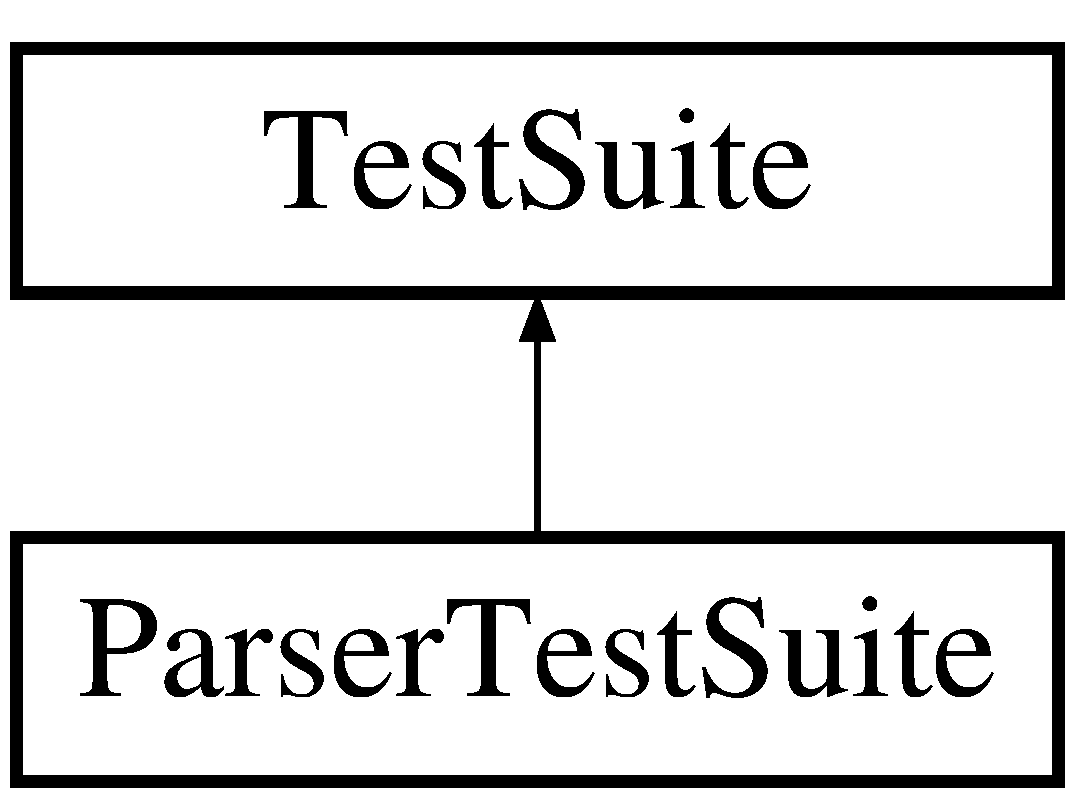
\includegraphics[height=2.000000cm]{class_parser_test_suite}
\end{center}
\end{figure}
\subsection*{Public Member Functions}
\begin{DoxyCompactItemize}
\item 
\hypertarget{class_parser_test_suite_ab7eff3217b5e28c9003f27c51da107ac}{}void {\bfseries test\+\_\+setup\+\_\+code} ()\label{class_parser_test_suite_ab7eff3217b5e28c9003f27c51da107ac}

\item 
\hypertarget{class_parser_test_suite_ac4a829a66a1582bee38e90ac3f0355f4}{}void {\bfseries test\+\_\+parse\+\_\+bad\+\_\+syntax} ()\label{class_parser_test_suite_ac4a829a66a1582bee38e90ac3f0355f4}

\item 
\hypertarget{class_parser_test_suite_a26eed485bc2671f4ac256ef97a21b704}{}void {\bfseries test\+\_\+parse\+\_\+sample\+\_\+1} ()\label{class_parser_test_suite_a26eed485bc2671f4ac256ef97a21b704}

\item 
\hypertarget{class_parser_test_suite_a0f1d6af1e07e35541fb83416d5e3e229}{}void {\bfseries test\+\_\+parse\+\_\+sample\+\_\+2} ()\label{class_parser_test_suite_a0f1d6af1e07e35541fb83416d5e3e229}

\item 
\hypertarget{class_parser_test_suite_aecc132f6b6dbb2e5bba08baec64f3f65}{}void {\bfseries test\+\_\+parse\+\_\+sample\+\_\+3} ()\label{class_parser_test_suite_aecc132f6b6dbb2e5bba08baec64f3f65}

\item 
\hypertarget{class_parser_test_suite_a6e5dfaf7b8ddc98001a4fec39b3f0a79}{}void {\bfseries test\+\_\+parse\+\_\+sample\+\_\+4} ()\label{class_parser_test_suite_a6e5dfaf7b8ddc98001a4fec39b3f0a79}

\item 
\hypertarget{class_parser_test_suite_a5b9a3cf2b76271244baaaaa4c8b7f7d5}{}void {\bfseries test\+\_\+parse\+\_\+sample\+\_\+5} ()\label{class_parser_test_suite_a5b9a3cf2b76271244baaaaa4c8b7f7d5}

\item 
\hypertarget{class_parser_test_suite_ae59d0f6d92f8d83833d51ef01479fdeb}{}void {\bfseries test\+\_\+parse\+\_\+mysample} ()\label{class_parser_test_suite_ae59d0f6d92f8d83833d51ef01479fdeb}

\item 
\hypertarget{class_parser_test_suite_a379db1a22b2c32defb8395b9b2166f76}{}void {\bfseries test\+\_\+parse\+\_\+forest\+Loss\+V2} ()\label{class_parser_test_suite_a379db1a22b2c32defb8395b9b2166f76}

\end{DoxyCompactItemize}
\subsection*{Public Attributes}
\begin{DoxyCompactItemize}
\item 
\hypertarget{class_parser_test_suite_a0c4943b3d23b79be363ba9e1ac7c02ed}{}\hyperlink{class_scanner}{Scanner} $\ast$ {\bfseries s}\label{class_parser_test_suite_a0c4943b3d23b79be363ba9e1ac7c02ed}

\item 
\hypertarget{class_parser_test_suite_a1d637f2f8be1326423ee5b4fd270c553}{}\hyperlink{class_parser}{Parser} $\ast$ {\bfseries p}\label{class_parser_test_suite_a1d637f2f8be1326423ee5b4fd270c553}

\end{DoxyCompactItemize}


The documentation for this class was generated from the following file\+:\begin{DoxyCompactItemize}
\item 
parser\+\_\+tests.\+h\end{DoxyCompactItemize}

\hypertarget{class_plus_sign_token}{}\section{Plus\+Sign\+Token Class Reference}
\label{class_plus_sign_token}\index{Plus\+Sign\+Token@{Plus\+Sign\+Token}}
Inheritance diagram for Plus\+Sign\+Token\+:\begin{figure}[H]
\begin{center}
\leavevmode
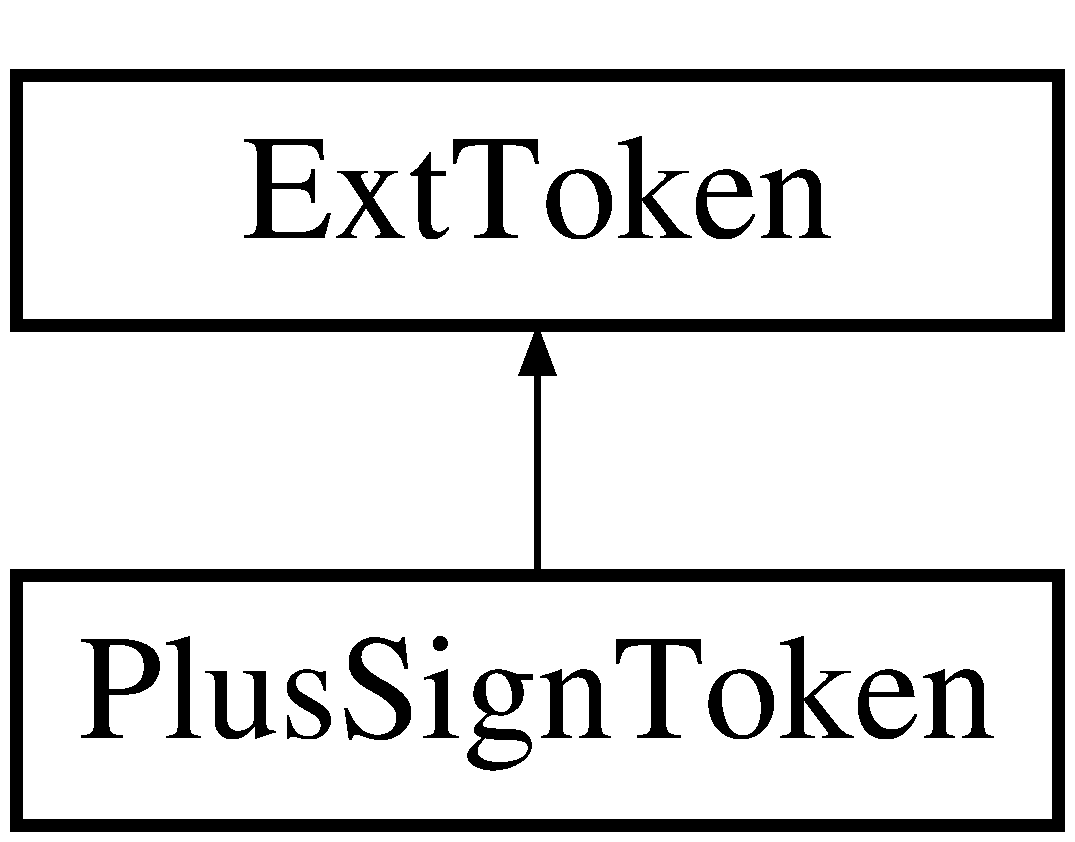
\includegraphics[height=2.000000cm]{class_plus_sign_token}
\end{center}
\end{figure}
\subsection*{Public Member Functions}
\begin{DoxyCompactItemize}
\item 
\hypertarget{class_plus_sign_token_ad480457c426f911f8286a73e8cf7f949}{}{\bfseries Plus\+Sign\+Token} (\hyperlink{class_parser}{Parser} $\ast$p, \hyperlink{class_token}{Token} $\ast$t)\label{class_plus_sign_token_ad480457c426f911f8286a73e8cf7f949}

\item 
\hypertarget{class_plus_sign_token_a4d79a17891f92800259308ce71402526}{}\hyperlink{class_parse_result}{Parse\+Result} {\bfseries led} (\hyperlink{class_parse_result}{Parse\+Result} left)\label{class_plus_sign_token_a4d79a17891f92800259308ce71402526}

\item 
\hypertarget{class_plus_sign_token_a61a05ac9660848e13da97d5746808868}{}std\+::string {\bfseries description} ()\label{class_plus_sign_token_a61a05ac9660848e13da97d5746808868}

\item 
\hypertarget{class_plus_sign_token_a80753eec970928e042da350df83150f2}{}int {\bfseries lbp} ()\label{class_plus_sign_token_a80753eec970928e042da350df83150f2}

\end{DoxyCompactItemize}
\subsection*{Additional Inherited Members}


The documentation for this class was generated from the following file\+:\begin{DoxyCompactItemize}
\item 
ext\+Token.\+h\end{DoxyCompactItemize}

\hypertarget{class_regex_test_suite}{}\section{Regex\+Test\+Suite Class Reference}
\label{class_regex_test_suite}\index{Regex\+Test\+Suite@{Regex\+Test\+Suite}}
Inheritance diagram for Regex\+Test\+Suite\+:\begin{figure}[H]
\begin{center}
\leavevmode
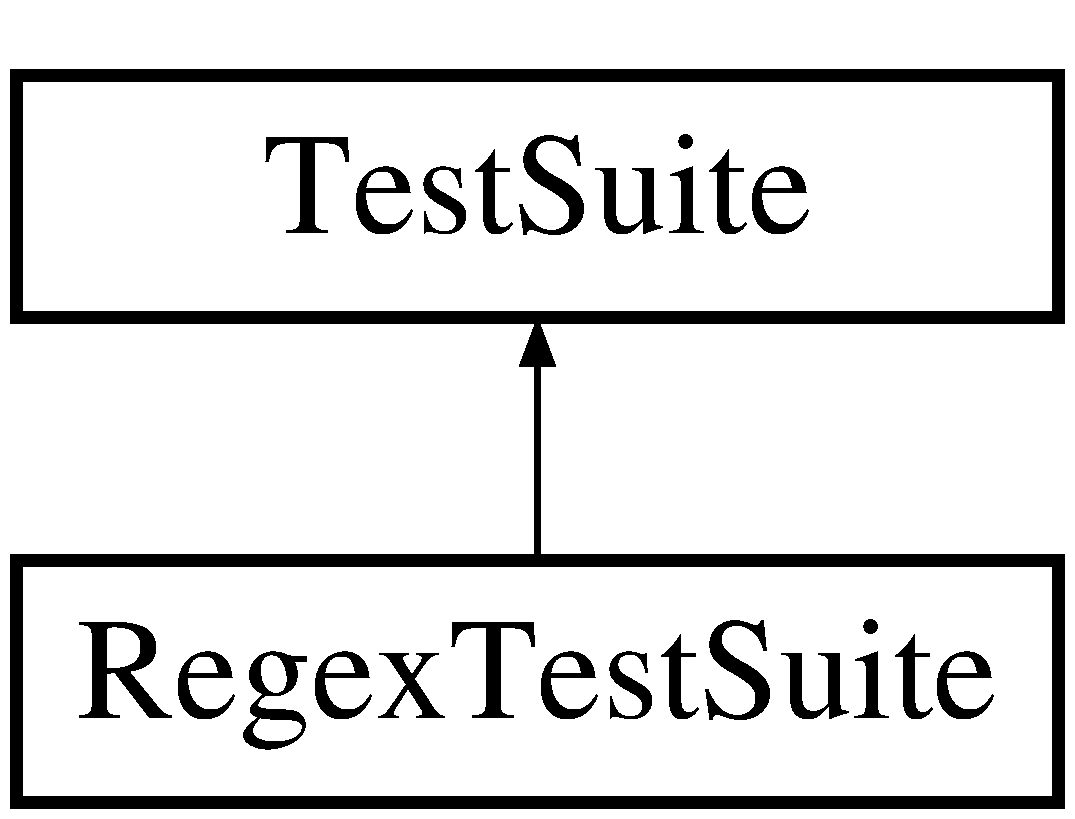
\includegraphics[height=2.000000cm]{class_regex_test_suite}
\end{center}
\end{figure}
\subsection*{Public Member Functions}
\begin{DoxyCompactItemize}
\item 
\hypertarget{class_regex_test_suite_aac0838d917fd9fd6cc71ee086c644555}{}void {\bfseries test\+\_\+make\+\_\+match\+Regex\+\_\+match} (void)\label{class_regex_test_suite_aac0838d917fd9fd6cc71ee086c644555}

\item 
\hypertarget{class_regex_test_suite_ad9c02b9f4fd7feca750d476cda8e0c60}{}void {\bfseries test\+\_\+make\+\_\+match\+Regex\+\_\+no\+\_\+match} (void)\label{class_regex_test_suite_ad9c02b9f4fd7feca750d476cda8e0c60}

\item 
\hypertarget{class_regex_test_suite_a0f46b90e2c0a1c98750a3335d086979a}{}void {\bfseries test\+\_\+make\+\_\+match\+Regex\+\_\+match\+\_\+string\+\_\+copy} (void)\label{class_regex_test_suite_a0f46b90e2c0a1c98750a3335d086979a}

\end{DoxyCompactItemize}


The documentation for this class was generated from the following file\+:\begin{DoxyCompactItemize}
\item 
regex\+\_\+tests.\+h\end{DoxyCompactItemize}

\hypertarget{class_relational_op_token}{}\section{Relational\+Op\+Token Class Reference}
\label{class_relational_op_token}\index{Relational\+Op\+Token@{Relational\+Op\+Token}}
Inheritance diagram for Relational\+Op\+Token\+:\begin{figure}[H]
\begin{center}
\leavevmode
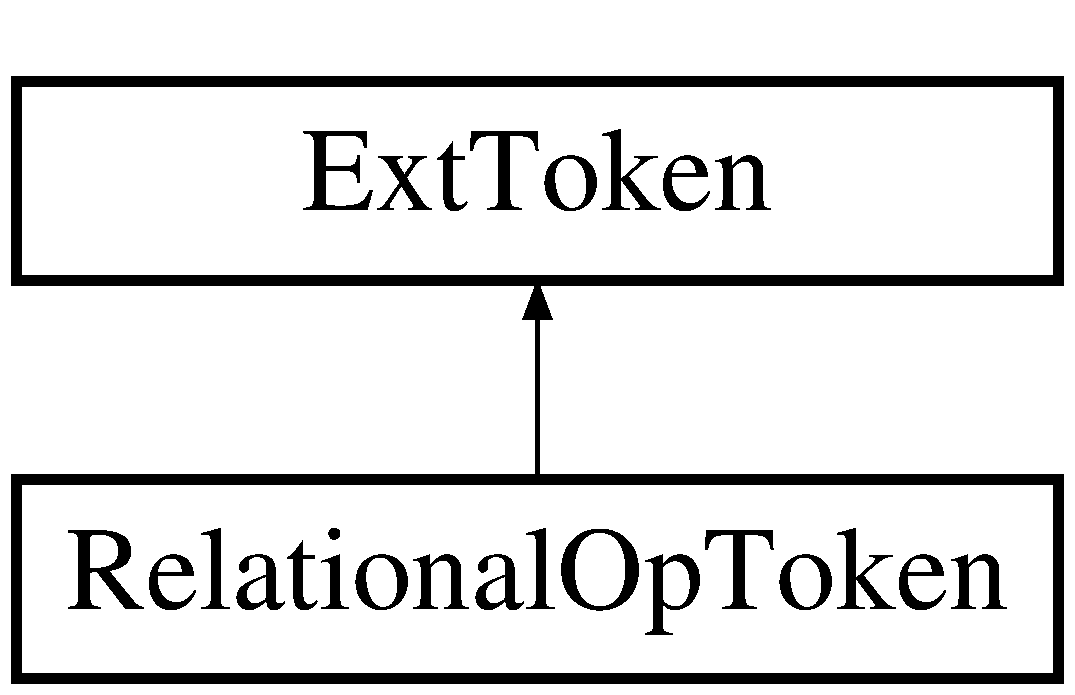
\includegraphics[height=2.000000cm]{class_relational_op_token}
\end{center}
\end{figure}
\subsection*{Public Member Functions}
\begin{DoxyCompactItemize}
\item 
\hypertarget{class_relational_op_token_a1ede45cf178138ff12beba209681be51}{}{\bfseries Relational\+Op\+Token} (\hyperlink{class_parser}{Parser} $\ast$p, \hyperlink{class_token}{Token} $\ast$t, std\+::string d)\label{class_relational_op_token_a1ede45cf178138ff12beba209681be51}

\item 
\hypertarget{class_relational_op_token_a426c64391e7b3272d8e6277964730e05}{}\hyperlink{class_parse_result}{Parse\+Result} {\bfseries led} (\hyperlink{class_parse_result}{Parse\+Result} left)\label{class_relational_op_token_a426c64391e7b3272d8e6277964730e05}

\item 
\hypertarget{class_relational_op_token_ada096491d9553aea21089230489d6aef}{}int {\bfseries lbp} ()\label{class_relational_op_token_ada096491d9553aea21089230489d6aef}

\end{DoxyCompactItemize}
\subsection*{Additional Inherited Members}


The documentation for this class was generated from the following file\+:\begin{DoxyCompactItemize}
\item 
ext\+Token.\+h\end{DoxyCompactItemize}

\hypertarget{class_scanner}{}\section{Scanner Class Reference}
\label{class_scanner}\index{Scanner@{Scanner}}
\subsection*{Public Member Functions}
\begin{DoxyCompactItemize}
\item 
\hypertarget{class_scanner_a4cf90c9e68bfb17f23af7368ff15766e}{}\hyperlink{class_token}{Token} $\ast$ {\bfseries scan} (const char $\ast$)\label{class_scanner_a4cf90c9e68bfb17f23af7368ff15766e}

\item 
\hypertarget{class_scanner_a9be26bf95e9661af0852a21fd311693d}{}\hyperlink{class_token}{Token} $\ast$ {\bfseries token\+Maker} (const char $\ast$)\label{class_scanner_a9be26bf95e9661af0852a21fd311693d}

\item 
\hypertarget{class_scanner_a47c391795bd333936f334f3a86b6e53e}{}bool {\bfseries token\+Maker\+\_\+bool} (token\+Type, const char $\ast$, const char $\ast$)\label{class_scanner_a47c391795bd333936f334f3a86b6e53e}

\item 
\hypertarget{class_scanner_ae9fb1d0074f17f291714b86097573058}{}regex\+\_\+t $\ast$ {\bfseries make\+Regex} (const char $\ast$)\label{class_scanner_ae9fb1d0074f17f291714b86097573058}

\item 
\hypertarget{class_scanner_ab873dc8eb3c741bec4634f055954ea97}{}int {\bfseries match\+Regex} (regex\+\_\+t $\ast$, const char $\ast$)\label{class_scanner_ab873dc8eb3c741bec4634f055954ea97}

\item 
\hypertarget{class_scanner_addc73cdb99ea3932ef130b6d17d920d9}{}int {\bfseries consume\+White\+Space\+And\+Comments} (regex\+\_\+t $\ast$, regex\+\_\+t $\ast$, regex\+\_\+t $\ast$, const char $\ast$)\label{class_scanner_addc73cdb99ea3932ef130b6d17d920d9}

\item 
\hypertarget{class_scanner_af660f8b4a17b79a75dd9ad35b5fcdcd3}{}void {\bfseries add\+To\+Array} (int, const char $\ast$, std\+::vector$<$ regex\+\_\+t $\ast$ $>$ \&expressions)\label{class_scanner_af660f8b4a17b79a75dd9ad35b5fcdcd3}

\end{DoxyCompactItemize}
\subsection*{Public Attributes}
\begin{DoxyCompactItemize}
\item 
\hypertarget{class_scanner_a2e2b865e62d926e58a16ba86c7288ea3}{}std\+::vector$<$ regex\+\_\+t $\ast$ $>$ {\bfseries expressions}\label{class_scanner_a2e2b865e62d926e58a16ba86c7288ea3}

\item 
\hypertarget{class_scanner_a2988e7836bc3fcf4b4593e82be3d50cf}{}std\+::vector$<$ regex\+\_\+t $\ast$ $>$ {\bfseries space\+Or\+Comment}\label{class_scanner_a2988e7836bc3fcf4b4593e82be3d50cf}

\end{DoxyCompactItemize}


The documentation for this class was generated from the following files\+:\begin{DoxyCompactItemize}
\item 
scanner.\+h\item 
scanner.\+cpp\end{DoxyCompactItemize}

\hypertarget{class_scanner_test_suite}{}\section{Scanner\+Test\+Suite Class Reference}
\label{class_scanner_test_suite}\index{Scanner\+Test\+Suite@{Scanner\+Test\+Suite}}
Inheritance diagram for Scanner\+Test\+Suite\+:\begin{figure}[H]
\begin{center}
\leavevmode
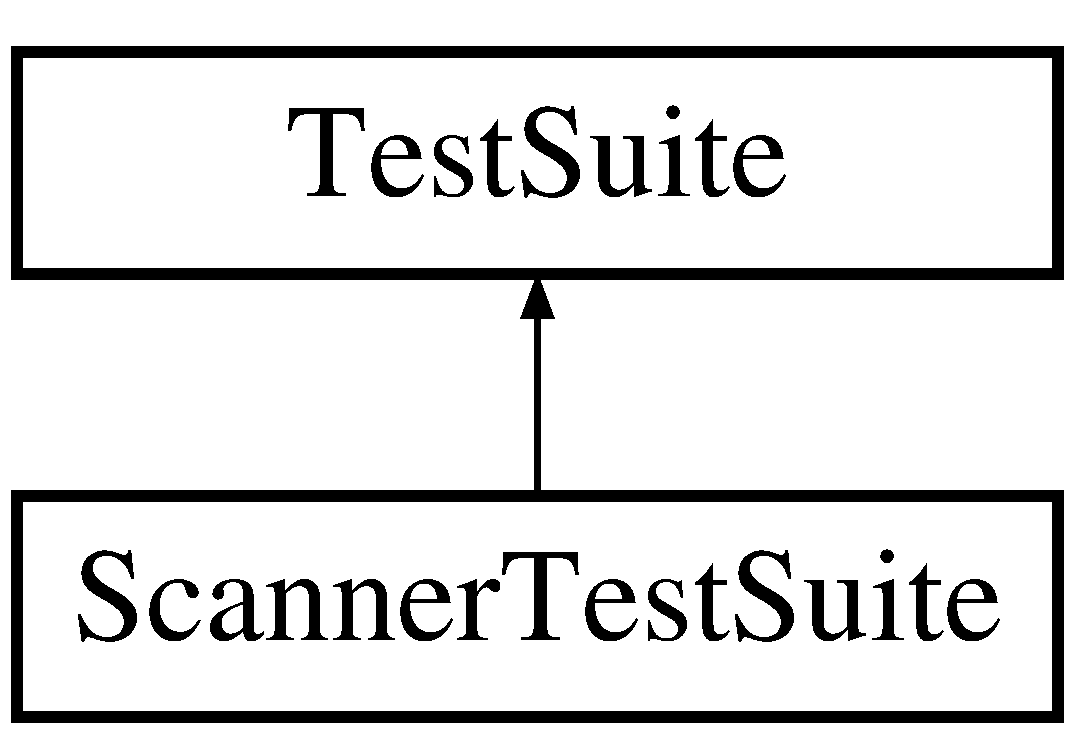
\includegraphics[height=2.000000cm]{class_scanner_test_suite}
\end{center}
\end{figure}
\subsection*{Public Member Functions}
\begin{DoxyCompactItemize}
\item 
\hypertarget{class_scanner_test_suite_ade832b9b4b3bd92980d43c4050cebd2c}{}void {\bfseries test\+\_\+setup\+\_\+code} ()\label{class_scanner_test_suite_ade832b9b4b3bd92980d43c4050cebd2c}

\item 
\hypertarget{class_scanner_test_suite_af42f8338bfe7b397ea39f565157f64cc}{}void {\bfseries test\+\_\+terminal\+\_\+int\+Kwd} ()\label{class_scanner_test_suite_af42f8338bfe7b397ea39f565157f64cc}

\item 
\hypertarget{class_scanner_test_suite_a5c55d99dbc84996abd740fbabb36314b}{}void {\bfseries test\+\_\+terminal\+\_\+float\+Kwd} ()\label{class_scanner_test_suite_a5c55d99dbc84996abd740fbabb36314b}

\item 
\hypertarget{class_scanner_test_suite_a919ec02392d67e0932affc229b1e72c8}{}void {\bfseries test\+\_\+terminal\+\_\+bool\+Kwd} ()\label{class_scanner_test_suite_a919ec02392d67e0932affc229b1e72c8}

\item 
\hypertarget{class_scanner_test_suite_a88607da81181c529df9b9edf246dfff6}{}void {\bfseries test\+\_\+terminal\+\_\+true\+Kwd} ()\label{class_scanner_test_suite_a88607da81181c529df9b9edf246dfff6}

\item 
\hypertarget{class_scanner_test_suite_a6a4395c74f53b0ff0024d6a81999d1b4}{}void {\bfseries test\+\_\+terminal\+\_\+false\+Kwd} ()\label{class_scanner_test_suite_a6a4395c74f53b0ff0024d6a81999d1b4}

\item 
\hypertarget{class_scanner_test_suite_a141d32b206981d44cbdbf478a20be967}{}void {\bfseries test\+\_\+terminal\+\_\+string\+Kwd} ()\label{class_scanner_test_suite_a141d32b206981d44cbdbf478a20be967}

\item 
\hypertarget{class_scanner_test_suite_ae2d7798c81ef50444efe99f5c7a89148}{}void {\bfseries test\+\_\+terminal\+\_\+matrix\+Kwd} ()\label{class_scanner_test_suite_ae2d7798c81ef50444efe99f5c7a89148}

\item 
\hypertarget{class_scanner_test_suite_aa35e7a92f4fdb1b6014ef0ca9df60ecc}{}void {\bfseries test\+\_\+terminal\+\_\+let\+Kwd} ()\label{class_scanner_test_suite_aa35e7a92f4fdb1b6014ef0ca9df60ecc}

\item 
\hypertarget{class_scanner_test_suite_a1f691532050a3925049694ca6776c08d}{}void {\bfseries test\+\_\+terminal\+\_\+in\+Kwd} ()\label{class_scanner_test_suite_a1f691532050a3925049694ca6776c08d}

\item 
\hypertarget{class_scanner_test_suite_ae4a9fa8bda3055d8704640f6308a80be}{}void {\bfseries test\+\_\+terminal\+\_\+end\+Kwd} ()\label{class_scanner_test_suite_ae4a9fa8bda3055d8704640f6308a80be}

\item 
\hypertarget{class_scanner_test_suite_a53ad312be41b5b2e01700f4ef35e3ed2}{}void {\bfseries test\+\_\+terminal\+\_\+if\+Kwd} ()\label{class_scanner_test_suite_a53ad312be41b5b2e01700f4ef35e3ed2}

\item 
\hypertarget{class_scanner_test_suite_accc9a3822b27c4abeadf5940954df2c6}{}void {\bfseries test\+\_\+terminal\+\_\+then\+Kwd} ()\label{class_scanner_test_suite_accc9a3822b27c4abeadf5940954df2c6}

\item 
\hypertarget{class_scanner_test_suite_a94ff796af7a2ff4dd70c04615767ab01}{}void {\bfseries test\+\_\+terminal\+\_\+else\+Kwd} ()\label{class_scanner_test_suite_a94ff796af7a2ff4dd70c04615767ab01}

\item 
\hypertarget{class_scanner_test_suite_a56ea8232db65862a9023cf0989940804}{}void {\bfseries test\+\_\+terminal\+\_\+for\+Kwd} ()\label{class_scanner_test_suite_a56ea8232db65862a9023cf0989940804}

\item 
\hypertarget{class_scanner_test_suite_a9a67154a3d7fd4888e5c4761065a460a}{}void {\bfseries test\+\_\+terminal\+\_\+while\+Kwd} ()\label{class_scanner_test_suite_a9a67154a3d7fd4888e5c4761065a460a}

\item 
\hypertarget{class_scanner_test_suite_a9c6323869bea7e4c738cedede8abf7a6}{}void {\bfseries test\+\_\+terminal\+\_\+print\+Kwd} ()\label{class_scanner_test_suite_a9c6323869bea7e4c738cedede8abf7a6}

\item 
\hypertarget{class_scanner_test_suite_a6f3d0ce7dbbd7f2a10d5223aa27db46e}{}void {\bfseries test\+\_\+terminal\+\_\+int\+Const} ()\label{class_scanner_test_suite_a6f3d0ce7dbbd7f2a10d5223aa27db46e}

\item 
\hypertarget{class_scanner_test_suite_a4b66e016244a602826a52db100b3628b}{}void {\bfseries test\+\_\+terminal\+\_\+float\+Const} ()\label{class_scanner_test_suite_a4b66e016244a602826a52db100b3628b}

\item 
\hypertarget{class_scanner_test_suite_ac6fbb996fdc378700e2c46512d3209e2}{}void {\bfseries test\+\_\+terminal\+\_\+string\+Const} ()\label{class_scanner_test_suite_ac6fbb996fdc378700e2c46512d3209e2}

\item 
\hypertarget{class_scanner_test_suite_a48ba8250d795af0d91f976bd32f67a30}{}void {\bfseries test\+\_\+terminal\+\_\+variable\+Name} ()\label{class_scanner_test_suite_a48ba8250d795af0d91f976bd32f67a30}

\item 
\hypertarget{class_scanner_test_suite_ac0e5e742c0384a39833b6f7bc71dd427}{}void {\bfseries test\+\_\+terminal\+\_\+left\+Paren} ()\label{class_scanner_test_suite_ac0e5e742c0384a39833b6f7bc71dd427}

\item 
\hypertarget{class_scanner_test_suite_afb533b7f05e10c3c5b418738dcac30a1}{}void {\bfseries test\+\_\+terminal\+\_\+right\+Paren} ()\label{class_scanner_test_suite_afb533b7f05e10c3c5b418738dcac30a1}

\item 
\hypertarget{class_scanner_test_suite_a4db81d5329c9c8d379ddab31626e94ab}{}void {\bfseries test\+\_\+terminal\+\_\+left\+Curly} ()\label{class_scanner_test_suite_a4db81d5329c9c8d379ddab31626e94ab}

\item 
\hypertarget{class_scanner_test_suite_ae493b914c95d91fdd0bf3119086e1873}{}void {\bfseries test\+\_\+terminal\+\_\+right\+Curly} ()\label{class_scanner_test_suite_ae493b914c95d91fdd0bf3119086e1873}

\item 
\hypertarget{class_scanner_test_suite_ad203f4631b835998a32530095cbfddf3}{}void {\bfseries test\+\_\+terminal\+\_\+left\+Square} ()\label{class_scanner_test_suite_ad203f4631b835998a32530095cbfddf3}

\item 
\hypertarget{class_scanner_test_suite_a178af38ac3787ec282cf4a6e471f42f8}{}void {\bfseries test\+\_\+terminal\+\_\+right\+Square} ()\label{class_scanner_test_suite_a178af38ac3787ec282cf4a6e471f42f8}

\item 
\hypertarget{class_scanner_test_suite_a31bf53c4955baf56480b24bf45e0c3de}{}void {\bfseries test\+\_\+terminal\+\_\+comma} ()\label{class_scanner_test_suite_a31bf53c4955baf56480b24bf45e0c3de}

\item 
\hypertarget{class_scanner_test_suite_abd07d9b6765ebe5315a3af872de282a4}{}void {\bfseries test\+\_\+terminal\+\_\+semi\+Colon} ()\label{class_scanner_test_suite_abd07d9b6765ebe5315a3af872de282a4}

\item 
\hypertarget{class_scanner_test_suite_a55c90b619b070f4239bdec72979bb5bf}{}void {\bfseries test\+\_\+terminal\+\_\+colon} ()\label{class_scanner_test_suite_a55c90b619b070f4239bdec72979bb5bf}

\item 
\hypertarget{class_scanner_test_suite_a8fbf222a7c786640d409c73bec29ee29}{}void {\bfseries test\+\_\+terminal\+\_\+assign} ()\label{class_scanner_test_suite_a8fbf222a7c786640d409c73bec29ee29}

\item 
\hypertarget{class_scanner_test_suite_a481065e6ca8656159bd055281c0f6823}{}void {\bfseries test\+\_\+terminal\+\_\+plus\+Sign} ()\label{class_scanner_test_suite_a481065e6ca8656159bd055281c0f6823}

\item 
\hypertarget{class_scanner_test_suite_a4a3dd116effbc9b2b137e847e0018c17}{}void {\bfseries test\+\_\+terminal\+\_\+star} ()\label{class_scanner_test_suite_a4a3dd116effbc9b2b137e847e0018c17}

\item 
\hypertarget{class_scanner_test_suite_ae4e04072daa5ae9e5372442642d10381}{}void {\bfseries test\+\_\+terminal\+\_\+dash} ()\label{class_scanner_test_suite_ae4e04072daa5ae9e5372442642d10381}

\item 
\hypertarget{class_scanner_test_suite_ae66a5c2bdbad866169648ead8a16bdbb}{}void {\bfseries test\+\_\+terminal\+\_\+forward\+Slash} ()\label{class_scanner_test_suite_ae66a5c2bdbad866169648ead8a16bdbb}

\item 
\hypertarget{class_scanner_test_suite_ada7c512cc23c4258c004283f215d0781}{}void {\bfseries test\+\_\+terminal\+\_\+less\+Than} ()\label{class_scanner_test_suite_ada7c512cc23c4258c004283f215d0781}

\item 
\hypertarget{class_scanner_test_suite_a018c232d0f36ba9096d3608230e20444}{}void {\bfseries test\+\_\+terminal\+\_\+less\+Than\+Equal} ()\label{class_scanner_test_suite_a018c232d0f36ba9096d3608230e20444}

\item 
\hypertarget{class_scanner_test_suite_ac951625ebf72efa7f3a5c23f7314508f}{}void {\bfseries test\+\_\+terminal\+\_\+greater\+Than} ()\label{class_scanner_test_suite_ac951625ebf72efa7f3a5c23f7314508f}

\item 
\hypertarget{class_scanner_test_suite_adfcd8e8afce3112198872f54a0ca2c2f}{}void {\bfseries test\+\_\+terminal\+\_\+greater\+Than\+Equal} ()\label{class_scanner_test_suite_adfcd8e8afce3112198872f54a0ca2c2f}

\item 
\hypertarget{class_scanner_test_suite_a4a15e77f16d68048c1a86ae078be2833}{}void {\bfseries test\+\_\+terminal\+\_\+equals\+Equals} ()\label{class_scanner_test_suite_a4a15e77f16d68048c1a86ae078be2833}

\item 
\hypertarget{class_scanner_test_suite_ac5ef06e31af6d84f45562beeae37cc0c}{}void {\bfseries test\+\_\+terminal\+\_\+not\+Equals} ()\label{class_scanner_test_suite_ac5ef06e31af6d84f45562beeae37cc0c}

\item 
\hypertarget{class_scanner_test_suite_ac59bf938e379950259fe3dcd7b49fc8e}{}void {\bfseries test\+\_\+terminal\+\_\+and\+Op} ()\label{class_scanner_test_suite_ac59bf938e379950259fe3dcd7b49fc8e}

\item 
\hypertarget{class_scanner_test_suite_a419f8b30aa9afc64a53dddac255429c2}{}void {\bfseries test\+\_\+terminal\+\_\+or\+Op} ()\label{class_scanner_test_suite_a419f8b30aa9afc64a53dddac255429c2}

\item 
\hypertarget{class_scanner_test_suite_a188e5bdd91f633e072957fd4e4944522}{}void {\bfseries test\+\_\+terminal\+\_\+not\+Op} ()\label{class_scanner_test_suite_a188e5bdd91f633e072957fd4e4944522}

\item 
\hypertarget{class_scanner_test_suite_a681db679ec2418f862f478fa7678942b}{}bool {\bfseries no\+Lexical\+Errors} (\hyperlink{class_token}{Token} $\ast$tks)\label{class_scanner_test_suite_a681db679ec2418f862f478fa7678942b}

\item 
\hypertarget{class_scanner_test_suite_a01dc6065a02127accc049627ae234129}{}void {\bfseries scan\+File\+No\+Lexical\+Errors} (const char $\ast$filename)\label{class_scanner_test_suite_a01dc6065a02127accc049627ae234129}

\item 
\hypertarget{class_scanner_test_suite_a97c50725866b3a5b36c36488053a59bc}{}bool {\bfseries same\+Terminals} (\hyperlink{class_token}{Token} $\ast$tks, int num\+Terms, token\+Type $\ast$ts)\label{class_scanner_test_suite_a97c50725866b3a5b36c36488053a59bc}

\item 
\hypertarget{class_scanner_test_suite_a01beafb44a33f4d80baf9a4208919c07}{}void {\bfseries test\+\_\+scan\+\_\+empty} ()\label{class_scanner_test_suite_a01beafb44a33f4d80baf9a4208919c07}

\item 
\hypertarget{class_scanner_test_suite_a304719dd961df0714d372010cdf99ef1}{}void {\bfseries test\+\_\+scan\+\_\+empty\+\_\+comment} ()\label{class_scanner_test_suite_a304719dd961df0714d372010cdf99ef1}

\item 
\hypertarget{class_scanner_test_suite_af85168e66ba2b924488aca9768231367}{}void {\bfseries test\+\_\+scan\+\_\+lexical\+Errors} ()\label{class_scanner_test_suite_af85168e66ba2b924488aca9768231367}

\item 
\hypertarget{class_scanner_test_suite_a4bd4d5fc2218f3d28b08b2821ecc271b}{}void {\bfseries test\+\_\+scan\+\_\+nums\+\_\+vars} ()\label{class_scanner_test_suite_a4bd4d5fc2218f3d28b08b2821ecc271b}

\item 
\hypertarget{class_scanner_test_suite_a5b47cd74d93c119b6f64b449fcc379f6}{}void {\bfseries xtest\+\_\+scan\+\_\+bad\+\_\+syntax\+\_\+good\+\_\+tokens} ()\label{class_scanner_test_suite_a5b47cd74d93c119b6f64b449fcc379f6}

\item 
\hypertarget{class_scanner_test_suite_a8248f8bda6c9909971ef13f1364ab8f8}{}void {\bfseries test\+\_\+scan\+\_\+sample\+\_\+forest\+Loss} ()\label{class_scanner_test_suite_a8248f8bda6c9909971ef13f1364ab8f8}

\end{DoxyCompactItemize}
\subsection*{Public Attributes}
\begin{DoxyCompactItemize}
\item 
\hypertarget{class_scanner_test_suite_a39987f3459098101d7c7fb5a4492996d}{}\hyperlink{class_scanner}{Scanner} $\ast$ {\bfseries s}\label{class_scanner_test_suite_a39987f3459098101d7c7fb5a4492996d}

\end{DoxyCompactItemize}


The documentation for this class was generated from the following file\+:\begin{DoxyCompactItemize}
\item 
scanner\+\_\+tests.\+h\end{DoxyCompactItemize}

\hypertarget{class_star_token}{}\section{Star\+Token Class Reference}
\label{class_star_token}\index{Star\+Token@{Star\+Token}}
Inheritance diagram for Star\+Token\+:\begin{figure}[H]
\begin{center}
\leavevmode
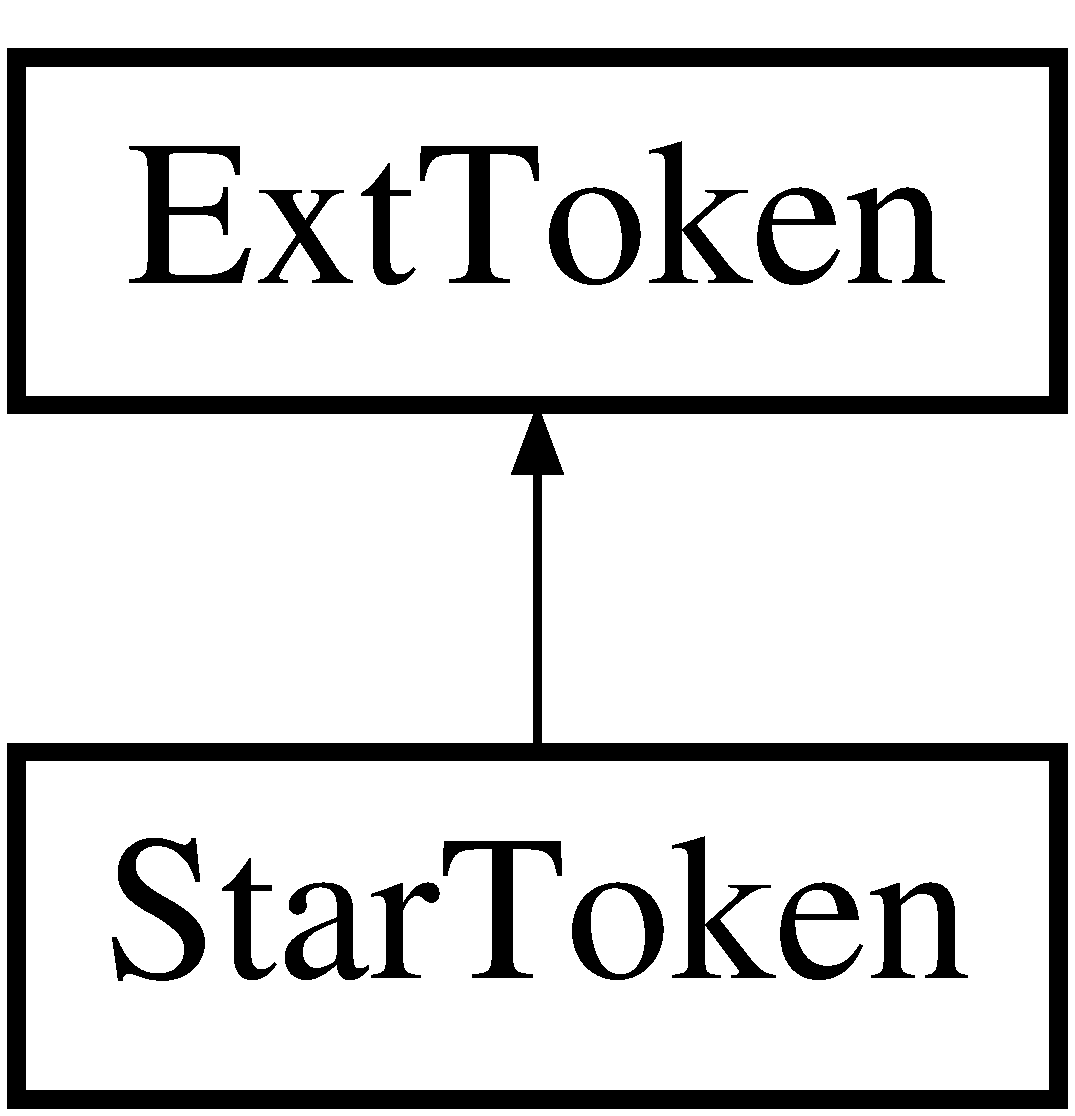
\includegraphics[height=2.000000cm]{class_star_token}
\end{center}
\end{figure}
\subsection*{Public Member Functions}
\begin{DoxyCompactItemize}
\item 
\hypertarget{class_star_token_a9e448a924eb2adbfde602c0590268afd}{}{\bfseries Star\+Token} (\hyperlink{class_parser}{Parser} $\ast$p, \hyperlink{class_token}{Token} $\ast$t)\label{class_star_token_a9e448a924eb2adbfde602c0590268afd}

\item 
\hypertarget{class_star_token_aba82bdc81500a58096bfeedad600ad10}{}\hyperlink{class_parse_result}{Parse\+Result} {\bfseries led} (\hyperlink{class_parse_result}{Parse\+Result} left)\label{class_star_token_aba82bdc81500a58096bfeedad600ad10}

\item 
\hypertarget{class_star_token_a59b81cb08057d75eca4b9a8aad8e2be1}{}std\+::string {\bfseries description} ()\label{class_star_token_a59b81cb08057d75eca4b9a8aad8e2be1}

\item 
\hypertarget{class_star_token_a87682a46d434781795d060e43e7eae23}{}int {\bfseries lbp} ()\label{class_star_token_a87682a46d434781795d060e43e7eae23}

\end{DoxyCompactItemize}
\subsection*{Additional Inherited Members}


The documentation for this class was generated from the following file\+:\begin{DoxyCompactItemize}
\item 
ext\+Token.\+h\end{DoxyCompactItemize}

\hypertarget{class_string_const_token}{}\section{String\+Const\+Token Class Reference}
\label{class_string_const_token}\index{String\+Const\+Token@{String\+Const\+Token}}
Inheritance diagram for String\+Const\+Token\+:\begin{figure}[H]
\begin{center}
\leavevmode
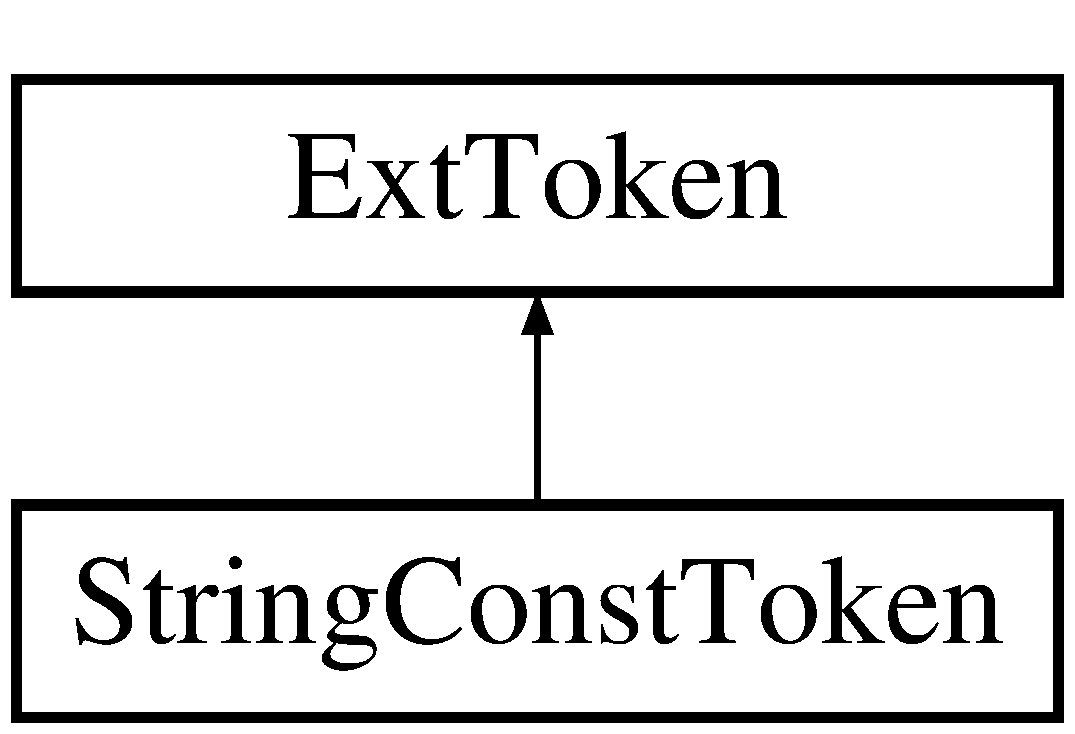
\includegraphics[height=2.000000cm]{class_string_const_token}
\end{center}
\end{figure}
\subsection*{Public Member Functions}
\begin{DoxyCompactItemize}
\item 
\hypertarget{class_string_const_token_aba75cdaef187138a572ba49a5c279fcf}{}{\bfseries String\+Const\+Token} (\hyperlink{class_parser}{Parser} $\ast$p, \hyperlink{class_token}{Token} $\ast$t)\label{class_string_const_token_aba75cdaef187138a572ba49a5c279fcf}

\item 
\hypertarget{class_string_const_token_a4767bba84d30289ab31d501f240b80fb}{}\hyperlink{class_parse_result}{Parse\+Result} {\bfseries nud} ()\label{class_string_const_token_a4767bba84d30289ab31d501f240b80fb}

\item 
\hypertarget{class_string_const_token_a6343169471a6cb6e422496f2f640691f}{}std\+::string {\bfseries description} ()\label{class_string_const_token_a6343169471a6cb6e422496f2f640691f}

\end{DoxyCompactItemize}
\subsection*{Additional Inherited Members}


The documentation for this class was generated from the following file\+:\begin{DoxyCompactItemize}
\item 
ext\+Token.\+h\end{DoxyCompactItemize}

\hypertarget{class_token}{}\section{Token Class Reference}
\label{class_token}\index{Token@{Token}}
\subsection*{Public Member Functions}
\begin{DoxyCompactItemize}
\item 
\hypertarget{class_token_a93748eebdfd09607d5170458c759d802}{}{\bfseries Token} (std\+::string, token\+Type, \hyperlink{class_token}{Token} $\ast$)\label{class_token_a93748eebdfd09607d5170458c759d802}

\end{DoxyCompactItemize}
\subsection*{Public Attributes}
\begin{DoxyCompactItemize}
\item 
\hypertarget{class_token_a1faf28f0fce064a0f34c7070ccd446a8}{}std\+::string {\bfseries lexeme}\label{class_token_a1faf28f0fce064a0f34c7070ccd446a8}

\item 
\hypertarget{class_token_a11b4722b5e4023d234d2017126de378b}{}token\+Type {\bfseries terminal}\label{class_token_a11b4722b5e4023d234d2017126de378b}

\item 
\hypertarget{class_token_a32f24a25af788c192e5b387dc8d67914}{}\hyperlink{class_token}{Token} $\ast$ {\bfseries next}\label{class_token_a32f24a25af788c192e5b387dc8d67914}

\end{DoxyCompactItemize}


The documentation for this class was generated from the following files\+:\begin{DoxyCompactItemize}
\item 
scanner.\+h\item 
scanner.\+cpp\end{DoxyCompactItemize}

\hypertarget{class_true_kwd_token}{}\section{True\+Kwd\+Token Class Reference}
\label{class_true_kwd_token}\index{True\+Kwd\+Token@{True\+Kwd\+Token}}
Inheritance diagram for True\+Kwd\+Token\+:\begin{figure}[H]
\begin{center}
\leavevmode
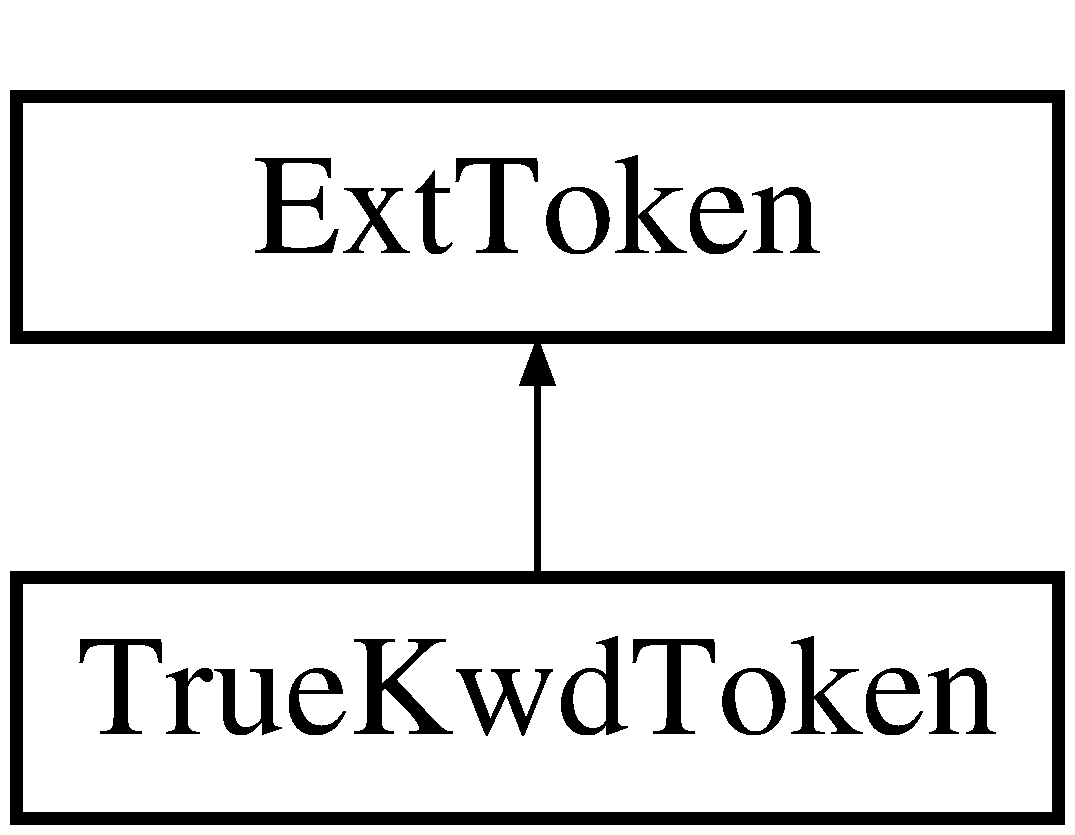
\includegraphics[height=2.000000cm]{class_true_kwd_token}
\end{center}
\end{figure}
\subsection*{Public Member Functions}
\begin{DoxyCompactItemize}
\item 
\hypertarget{class_true_kwd_token_aec070f83a6b91ed35a41e24dfd301b17}{}{\bfseries True\+Kwd\+Token} (\hyperlink{class_parser}{Parser} $\ast$p, \hyperlink{class_token}{Token} $\ast$t)\label{class_true_kwd_token_aec070f83a6b91ed35a41e24dfd301b17}

\item 
\hypertarget{class_true_kwd_token_ad86f05acb9483438db153eab44aa6dac}{}\hyperlink{class_parse_result}{Parse\+Result} {\bfseries nud} ()\label{class_true_kwd_token_ad86f05acb9483438db153eab44aa6dac}

\item 
\hypertarget{class_true_kwd_token_af4dbe740f06e6928a436d06349af67a9}{}std\+::string {\bfseries description} ()\label{class_true_kwd_token_af4dbe740f06e6928a436d06349af67a9}

\end{DoxyCompactItemize}
\subsection*{Additional Inherited Members}


The documentation for this class was generated from the following file\+:\begin{DoxyCompactItemize}
\item 
ext\+Token.\+h\end{DoxyCompactItemize}

\hypertarget{class_variable_name_token}{}\section{Variable\+Name\+Token Class Reference}
\label{class_variable_name_token}\index{Variable\+Name\+Token@{Variable\+Name\+Token}}
Inheritance diagram for Variable\+Name\+Token\+:\begin{figure}[H]
\begin{center}
\leavevmode
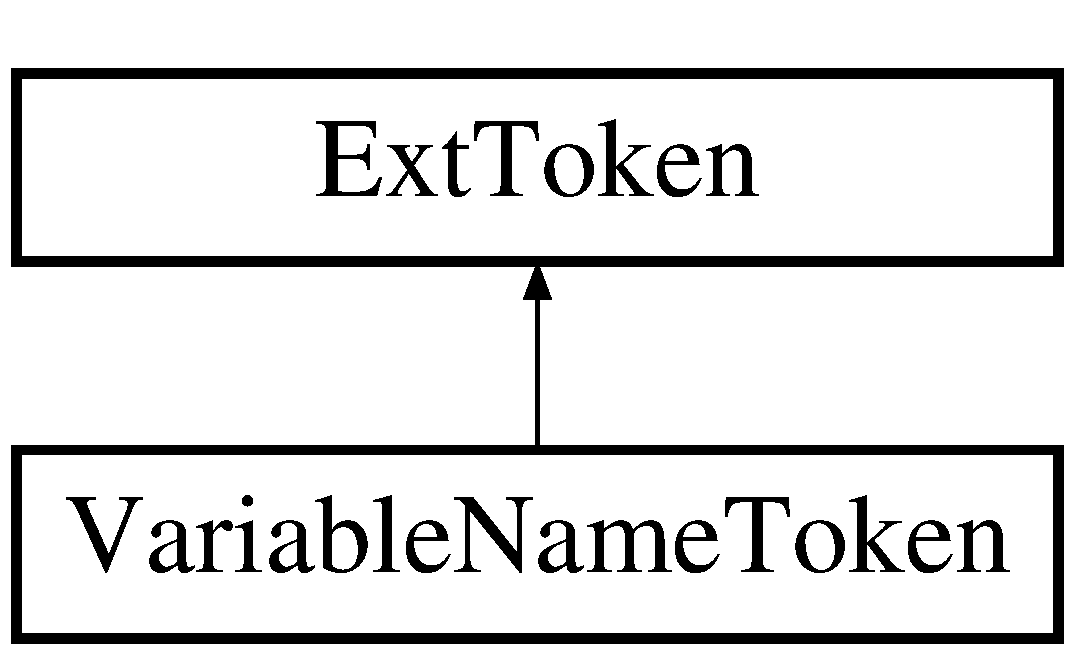
\includegraphics[height=2.000000cm]{class_variable_name_token}
\end{center}
\end{figure}
\subsection*{Public Member Functions}
\begin{DoxyCompactItemize}
\item 
\hypertarget{class_variable_name_token_a804403db425122d1c8d40fd2c6172439}{}{\bfseries Variable\+Name\+Token} (\hyperlink{class_parser}{Parser} $\ast$p, \hyperlink{class_token}{Token} $\ast$t)\label{class_variable_name_token_a804403db425122d1c8d40fd2c6172439}

\item 
\hypertarget{class_variable_name_token_a6e775ad5b8c2eafd2e2a185ab90b1f27}{}\hyperlink{class_parse_result}{Parse\+Result} {\bfseries nud} ()\label{class_variable_name_token_a6e775ad5b8c2eafd2e2a185ab90b1f27}

\item 
\hypertarget{class_variable_name_token_a54bc3a78736e5c967dc4b1c58e66135b}{}std\+::string {\bfseries description} ()\label{class_variable_name_token_a54bc3a78736e5c967dc4b1c58e66135b}

\end{DoxyCompactItemize}
\subsection*{Additional Inherited Members}


The documentation for this class was generated from the following file\+:\begin{DoxyCompactItemize}
\item 
ext\+Token.\+h\end{DoxyCompactItemize}

%--- End generated contents ---

% Index
\backmatter
\newpage
\phantomsection
\clearemptydoublepage
\addcontentsline{toc}{chapter}{Index}
\printindex

\end{document}
